\documentclass[twoside]{article}

\usepackage[accepted]{aistats2025}




\usepackage{wrapfig}

% If you use the following package, be sure to comment out \usepackate{xcolor}

\usepackage{multirow,mathtools } \usepackage{algorithm,algpseudocode}

% Very useful for various special symbols
\usepackage{pifont}
% For \rowcolor
\usepackage{color, colortbl}

\usepackage{blindtext}
\usepackage{lipsum}

\usepackage{multirow}
\usepackage{graphicx}
\usepackage{listings}

\usepackage{bbm}
\usepackage{dsfont}

\usepackage[most]{tcolorbox}

\newcommand{\JH}[1]{\textcolor{blue}{JH: #1}}
\newcommand{\SL}[1]{\textcolor{purple}{SL: #1}}
\newcommand{\JC}[1]{\textcolor{cyan}{JC: #1}}
\newcommand{\SM}[1]{\textcolor{red}{SM: #1}}
\newcommand{\CF}[1]{\textcolor{orange}{CF: #1}}
\newcommand{\RZ}[1]{\textcolor{red}{RZ: #1}}
\newcommand{\LL}[1]{\textcolor{red}{LL: #1}}
\newcommand{\YY}[1]{\textcolor{red}{YY: #1}}

%%%%% NEW MATH DEFINITIONS %%%%%

% \usepackage{amsmath,amsfonts,bm}
\usepackage{amsmath,amsfonts}

\usepackage{pifont}


\newcommand{\R}{\mathbb{R}}


\def\va{{\mathbf{a}}}
\def\vg{{\mathbf{g}}}

% Sets
\def\sR{\mathbb{R}}
\def\sC{\mathbb{C}}
\def\sZ{\mathbb{Z}}
\def\sN{\mathbb{N}}
\def\sQ{\mathbb{Q}}

\def\sS{\mathcal{S}}



% Vectors
\def\vzero{{\mathbf{0}}}
\def\vone{{\mathbf{1}}}
\def\vmu{{\mathbf{\mu}}}
\def\vtheta{{\mathbf{\theta}}}
\def\va{{\mathbf{a}}}
\def\vb{{\mathbf{b}}}
\def\vc{{\mathbf{c}}}
\def\vd{{\mathbf{d}}}
\def\ve{{\mathbf{e}}}
\def\vf{{\mathbf{f}}}
\def\vg{{\mathbf{g}}}
\def\vh{{\mathbf{h}}}
\def\vi{{\mathbf{i}}}
\def\vj{{\mathbf{j}}}
\def\vk{{\mathbf{k}}}
\def\vl{{\mathbf{l}}}
\def\vm{{\mathbf{m}}}
\def\vn{{\mathbf{n}}}
\def\vo{{\mathbf{o}}}
\def\vp{{\mathbf{p}}}
\def\vq{{\mathbf{q}}}
\def\vr{{\mathbf{r}}}
\def\vs{{\mathbf{s}}}
\def\vt{{\mathbf{t}}}
\def\vu{{\mathbf{u}}}
\def\vv{{\mathbf{v}}}
\def\vw{{\mathbf{w}}}
\def\vx{{\mathbf{x}}}
\def\vy{{\mathbf{y}}}
\def\vz{{\mathbf{z}}}
\def\vzeta{{\mathbf{\zeta}}}

% Matrix
\def\mA{{\mathbf{A}}}
\def\mB{{\mathbf{B}}}
\def\mC{{\mathbf{C}}}
\def\mD{{\mathbf{D}}}
\def\mE{{\mathbf{E}}}
\def\mF{{\mathbf{F}}}
\def\mG{{\mathbf{G}}}
\def\mH{{\mathbf{H}}}
\def\mI{{\mathbf{I}}}
\def\mJ{{\mathbf{J}}}
\def\mK{{\mathbf{K}}}
\def\mL{{\mathbf{L}}}
\def\mM{{\mathbf{M}}}
\def\mN{{\mathbf{N}}}
\def\mO{{\mathbf{O}}}
\def\mP{{\mathbf{P}}}
\def\mQ{{\mathbf{Q}}}
\def\mR{{\mathbf{R}}}
\def\mS{{\mathbf{S}}}
\def\mT{{\mathbf{T}}}
\def\mU{{\mathbf{U}}}
\def\mV{{\mathbf{V}}}
\def\mW{{\mathbf{W}}}
\def\mX{{\mathbf{X}}}
\def\mY{{\mathbf{Y}}}
\def\mZ{{\mathbf{Z}}}
\def\mBeta{{\mathbf{\beta}}}
\def\mPhi{{\mathbf{\Phi}}}
\def\mLambda{{\mathbf{\Lambda}}}
\def\mSigma{{\mathbf{\Sigma}}}


% Expectation
% \def\eE{\mathop{\mathbb{E}}\limits}
\def\eE{\mathbb{E}}

% Probability
\def\pP{\mathbb{P}}

% Tilde
\def\tf{\tilde{f}}
\def\tS{\tilde{S}}
\def\wtF{\widetilde{\mathcal{F}}}
\def\whR{\widehat{R}}
\def\tvx{\tilde{\mathbf{x}}}
\def\ty{\tilde{y}}


\def\defeq{\overset{\textup{def}}{=}}
% \def\defeq{\overset{.}{=}}
\def\defone{\overset{\text{\ding{172}}}{=}}
\def\deftwo{\overset{\text{\ding{173}}}{=}}
\def\leqone{\overset{\text{\ding{172}}}{\leq}}
\def\leqtwo{\overset{\text{\ding{173}}}{\leq}}
\def\leqthree{\overset{\text{\ding{174}}}{\leq}}
\def\leqfour{\overset{\text{\ding{175}}}{\leq}}
\def\eqone{\overset{\text{\ding{172}}}{=}}
\def\eqtwo{\overset{\text{\ding{173}}}{=}}
\def\eqthree{\overset{\text{\ding{174}}}{=}}
\def\eqfour{\overset{\text{\ding{175}}}{=}}
\def\geqfive{\overset{\text{\ding{176}}}{\geq}}


\usepackage{dirtytalk} %
\usepackage{hyperref} %

\hypersetup{
    colorlinks,
    linkcolor={black},
    citecolor={black},
    urlcolor={black}
}
\usepackage{booktabs} %


\usepackage[round]{natbib}
\bibliographystyle{plainnat}
\renewcommand{\bibname}{References}
\renewcommand{\bibsection}{\subsubsection*{\bibname}}

\usepackage{xr-hyper}

\setlength{\textfloatsep}{11pt}
\setlength{\floatsep}{15pt}
\begin{document}


\runningauthor{P. Bevanda, M. Beier, A. Lederer, A. Capone, S. Sosnowski, S. Hirche}


\twocolumn[

\aistatstitle{Koopman-Equivariant Gaussian Processes}


\aistatsauthor{Petar Bevanda$^{*}$ \\ TU Munich \And Max Beier$^{*}$ \\ TU Munich
\And Alexandre Capone \\ CMU Robotics Institute \AND Stefan Sosnowski \\ TU Munich \And Sandra Hirche \\ TU Munich \And Armin Lederer \\ ETH Z\"{u}rich 
}
\aistatsaddress{} 
]

\begin{abstract}
Credible forecasting and representation learning of dynamical systems are of ever-increasing importance for reliable decision-making. To that end, we propose a family of Gaussian processes (GP) for dynamical systems with linear time-invariant responses, which are nonlinear only in initial conditions. This linearity allows us to tractably quantify forecasting and
representational uncertainty, simultaneously alleviating the challenge of computing the distribution of trajectories from a GP-based dynamical system and enabling a new probabilistic treatment of learning Koopman operator representations. Using a trajectory-based equivariance -- which we refer to as \textit{Koopman equivariance} -- we obtain a  GP model with enhanced generalization capabilities. To allow for large-scale regression, we equip our framework with variational inference based on suitable inducing points. Experiments demonstrate on-par and often better forecasting performance compared to kernel-based methods for learning dynamical systems.
\end{abstract}


\section{INTRODUCTION}
Learning predictive models for forecasting dynamic systems is a challenging task due to complex and often unknown interactions between quantities of interest \citep{Brunton2019Data-DrivenEngineering}. The great utility of such models helps advance various different fields such as fluid mechanics \citep{kundu2015fluid}, molecular biology \citep{protFold}, robotics \citep{Billard2022LearningApproach} or safety-constrained decision making \citep{Hewing/annurev-control-090419-075625, Brunke/annurev-control-042920-020211}.
Dynamical system descriptions commonly require simulation for forecasting and uncertainty propagation, which can be difficult for non-parametric data-driven models \citep{pmlr-v120-hewing20a,TBpredGP}. 
In most real-world applications involving dynamical systems,  
measurements often come in the form of sequential one-step transition data that is sampled arbitrarily and potentially non-uniformly. Furthermore, there is often a certain regularity in the evolution of quantities of interest \citep{pmlr-v202-bilos23a} across domains \citep{SEZER2020106181,DEB2017902,Lim2021}, making it important to impose structure that discourages temporal fluctuations. 
To account for these different challenges in modeling dynamical systems, the choice of \textit{representations} when learning from data becomes a deciding factor in the difficulty of forecasting as well as inference, especially when modeling complex phenomena \citep{Mezic2004ComparisonBehavior} or long time-series \citep{DBLP:conf/iclr/GuGR22}.
In this paper, we focus on non-parametric learning paradigms, emphasizing \textit{uncertainty quantification} and \textit{forecasting simplicity}. In particular, we study the interplay between Gaussian processes \citep{Rasmussen2006} and effective dynamical system linearizations based on Koopman operators \citep{KoopBook,Brunton2022ModernSystems}. A more exhaustive account of related work is delegated to the supplementary material.
\begin{table}[t!]%
    \caption{Nonlinear dynamics modeling from data}
    \label{tab:contribution}
    \footnotesize
    \centering
    \vspace{-2ex}
    \begin{tabular}{l|ccccc}
    \toprule
        Approach& LTI forecast & End-to-end & Bayesian\\
        \midrule
        GPs & \color{red!80!black}{\text{\xmark}}  & \color{green!80!black}{\text{\cmark}} & \color{green!80!black}{\text{\cmark}}\\
        Koopman & \color{green!80!black}{\text{\cmark}}  & \color{red!80!black}{\text{\xmark}} & \color{red!80!black}{\text{\xmark}} \\
        {{\tbm{this work}}} & \color{green!80!black}{\text{\cmark}} & \color{green!80!black}{\text{\cmark}} & \color{green!80!black}{\text{\cmark}} \\
        \bottomrule
    \end{tabular}
\end{table}

\textbf{Gaussian processes.~~}
Gaussian processes (GPs) \citep{Rasmussen2006} have the capability of inferring models with little structural prior knowledge: either by using so-called universal kernels \citep{Micchelli2006UniversalKernels} or placing a prior on a set of kernels and optimizing their likelihood \citep{Duvenaud2014}. 
In particular, their ability to quantify epistemic uncertainty has led to a common application in safety-critical control problems \citep{BerkenkampECC15,pmlr-v37-sui15,NIPS2017_766ebcd5,CuriCDC22,Baumann2021,Khosravi2023bo,As2024,Polymenakos2020,Lederer2021GaussianApplications}. Commonly employed as single-step predictors, GP models necessitate approximations for predicting probability distributions that go beyond a single time-step into the future. Thus, dealing with multi-step prediction often relies on iterative sampling-based approaches \citep{Bradford2019,pmlr-v120-hewing20a, TBpredGP} that are generally computationally expensive.
Alternatively, one can employ methods of reduced computational complexity, such as Taylor approximations \citep{Girard2003} or exact moment matching \citep{Deisenroth2011PILCO:Search}. However, such approaches deliver no accuracy guarantees for long-term forecasts. Notably, one can avoid approximate uncertainty propagation via multitask GPs models \citep{Bonilla2007} that use a collection of ``condensed models", one for each of the prediction steps \citep{Bradford2019,Pfefferkorn2022}, or employ a single contextual kernel defined over a joint spatio-temporal domain \citep{pmlr-v151-zenati22a, Li2024STkernel}.\looseness=-1

\textbf{Koopman operator-based learning.~~}
The linearity of Koopman operators and the forecasting simplicity of \textit{linear time-invariant} (LTI) models stemming from their eigendecompositions has led to their increasing popularity in learning dynamical systems \citep{Bevanda2021KoopmanControl,Otto2021AnnualSystems,Brunton2022ModernSystems}. 
Nevertheless, existing LTI predictors based on operator regression are limited to dissecting long-term components of ergodic dynamics \citep{Korda2018OnOperator,Klus2020EigendecompositionsSpaces,Kostic2022LearningSpaces,Kostic2023KoopmanEigenvalues}. While this approach is extremely powerful for stationary data and reversible dynamics, almost all real-world dynamical systems are irreversible and often even nonstationary \citep{Wu2020}.
Thus, an increasing amount of methods considers kernels that are \textit{dynamics-informed} \citep{Zhao_2016,BERRY2016439,Banisch2017,ALEXANDER2020132520,Burov2021,DUFEE2024134044}. By plugging samples of the dynamics from sequential data into the kernel itself, eigenfunctions of Koopman operators can be directly accessed for both ergodic \citep{DUFEE2024134044} and transient settings \citep{KKR_neurips2023}.~
While the latter has generalization and consistency guarantees, fully tractable representational uncertainty is impossible due to a two-stage regression approach \citep{HarmlessEcon,Wang2022}. Still, the existing Koopman operator-based learning approaches offer no epistemic uncertainty bounds, principled model selection or handling of observation noise.

In this work, we present \textbf{K}oopman-\textbf{E}quivariant \textbf{G}aussian \textbf{P}rocesses (KE-GPs), the first universal GP models with fully tractable and closed-form confidence bounds for multi-step prediction. By leveraging latent dynamics, our model provides simple LTI responses as a nonlinear function of the initial condition. Strikingly, our GP model provides enhanced generalization compared to existing methods due to intrinsic symmetries (Koopman-equivariants). Furthermore, it delivers continuous-time posteriors without requiring time-derivative data. KE-GPs allow for tractable \textit{simultaneous characterization of both forecasting and representational uncertainty} – alleviating a traditional
challenge of GPs and enabling a novel probabilistic treatment of learning dynamics representations.\footnote{{\textbf{Notation:} Denote the joint data distribution as $P(d z \times d x \times d y)$, its marginal distributions as $P(d x), P(d z)$, etc., and their support as $\mathcal{X}, \mathcal{Z}$. For functions of observed variables (e.g., $\bm{x}$ or z), $\|\cdot\|_2$ denotes the $L_2$ norm w.r.t. the respective marginal data distribution. $\|\cdot\|_{\infty}$ denotes the $L_{\infty}$ norm. We use the notation $[m]:=\{1, \ldots, m\}$. Boldface $(\bm{x}, \bm{y}, \bm{z})$ emphasizes the denotation of random variables. For any kernel $k, \mathcal{G} \mathcal{P}(0, k)$ refers to the ``standard Gaussian process" \citep{vanderVaart2008} with zero mean, and covariance defined by $k . \lesssim, \gtrsim, \asymp$ represent (in)equalities up to constants; the hidden constants will not depend on any sample size. $\tilde{\mathcal{O}}(\cdot)$ denotes inequality up to logarithm factors.}}



\textbf{Organization\footnote{Proofs of theoretical results are in the supplemental.}.}
In Section \ref{sec:ProbStat} we introduce the necessary preliminaries together with our problem statement.
    Section \ref{sec:KEframework} includes the derivation of Koopman-equivariant Gaussian process models, including representation theory and dynamical properties. We then analyze the sample-complexity of our approach through an information-theoretical lens, in Section \ref{section:analysisofsamplecomplexity}.
To handle large datasets, in Section \ref{section:svigps}, we present our Koopman-equivariant inducing variables for scalable GP-based modeling using variational inference.
In Section \ref{sec:NumExp} we demonstrate the utility of our KE-GP approach through a comparison to existing GP and Koopman approaches for learning dynamical systems
including predator-prey ODE, datasets from realistic robotic simulators as well as real-world weather data. 
Finally, in Section \ref{sec:Concl}, we conclude and mention the limitations of the approach.\looseness=-1
\section{PROBLEM SETTING}\label{sec:ProbStat}
Our work builds upon the extensive literature on GPs, their interplay with linear operators, and the concept of Koopman-equivariance, which extracts informative ``latent states" of dynamics, i.e., Koopman operator eigenfunctions, based on trajectory data. The following covers the necessary prerequisites for setting up the interplay between GPs, linear operators, and intrinsic dynamical system symmetries.
\subsection{Gaussian Process Regression}\label{sec:BackgroundGPs}
A Gaussian process is a generalization of the Gaussian distribution. It specifies a distribution, such that any finite collection of random variables follows a joint Gaussian distribution, which can be interpreted as a distribution over functions $f:\mathbb{R}^n\rightarrow\mathbb{R}$ commonly denoted by $f(\cdot)\sim\GP(m(\cdot),k(\cdot,\cdot))$ \citep{Rasmussen2006}. This distribution is defined using a prior mean function $m:\mathbb{R}^n\rightarrow\mathbb{R}$ and a covariance function $k:\mathbb{R}^n\times\mathbb{R}\rightarrow\mathbb{R}_{0,+}$. The mean function $m(\cdot)$ includes prior models and is often set to $0$ in the absence of such information, which we also assume in the following. The covariance function $k(\cdot,\cdot)$ encodes more abstract prior knowledge, such as symmetries and smoothness of the sample functions.

Given a dataset $\mathbb{D}_N=\{\bm{z}^{(i)},y^{(i)} \}_{i\in[N]}$ with training targets $y^{(i)}=f(\bm{z}^{(i)})+\omega^{(i)}$ perturbed by i.i.d. Gaussian noise $\omega^{(i)}\sim\mathcal{N}(0,\sigma_{\txt{on}}^2)$, we place a Gaussian process prior $\GP(0,k(\cdot,\cdot))$ on the unknown function $f(\cdot)$ to infer a model. This is straightforwardly achieved by computing the posterior distribution given the training data, which is Gaussian at each test point $\bm{z}\in\mathbb{R}^n$. We can then compactly express the posterior as $p(f(\bm{z})|\mathbb{D}_N)=\mathcal{N}(\mu(\bm{z}),\sigma^2(\bm{z}))$, where 
\begin{align}\label{eq:GPbase}
 \textstyle   \mu(\bm{z})&=\bm{k}^{\intercal}(\bm{z})(\bm{K}+\sigma_n^2\bm{I})^{-1}\bm{y},\\
    \sigma^2(\bm{z})&=k(\bm{z},\bm{z})-\bm{k}^{\intercal}(\bm{z})(\bm{K}+\sigma_{\txt{on}}^2\bm{I}_N)^{-1}\bm{k}(\bm{z}),
\end{align}
with $k_i(\bm{z})=k(\bm{z},\bm{z}^{(i)})$, $K_{ij}=k(\bm{z}^{(i)},\bm{z}^{(j)})$ and $\bm{y}^\intercal=[y^{(1)}\ \cdots\ y^{(N)}]$. In addition to inferring the posterior distribution, we use the training data to optimize the hyperparameters that arise from the kernel parameterization. This is enabled by the probabilistic approach to the regression problem, which allows us to choose the hyperparameters by minimizing the negative log-likelihood $\textstyle  -\log (p(\bm{y}|\bm{Z}))= \textstyle \nicefrac{1}{2}\bm{y}^{\intercal}(\bm{K}+\sigma_{\txt{on}}^2\bm{I}_N)^{-1}\bm{y}+\nicefrac{1}{2}\log(\det(\bm{K}+\sigma_{\txt{on}}^2\bm{I}_N))+\nicefrac{N}{2}\log(2\pi)$.

\subsection{System Class \& Modeling Approach}
\textbf{System class.~~} We consider state-space models
\begin{taggedsubequations}{\txt{SSM}}\label{eq:SSmodel}
\begin{align}
\text{(dynamics)}  \qquad  \dot{\bm{x}}&=\bm{f}
(\bm{x}), \quad \bm{x} \in \Set{X} \subset \RR^n, \quad \label{eq:SSMdyn}\\
\text{(output)}   \qquad    y&=h(\bm{x}) \in \RR, \quad \label{eq:SSMout}
\end{align}
\end{taggedsubequations}%
with a well-defined flow $\bm{F}_{t}(\bm{x}{\naught}):=\normalint_0^{t} \bm{f}(\bm{x}(\tau)) d\tau$ that requires local Lipschitz continuity of $\bm{f}$, which is natural to physical systems that often evolve ``smoothly''.
The canonical forecasting model for \eqref{eq:SSmodel} is $y(t,\bm{x}_0) := h_t(\bm{x}_0)\equiv h \circ \bm{F}_{t}(\bm{x}_0)$. In practice, a numerical integration scheme is usually required to solve the integral for a shorter time-interval ${\Delta}{t}$, such that the actual forecast becomes an $H$-fold composition of nonlinear maps $\textstyle y(t,\bm{x}_0) \approx \textstyle h \circ \bm{F}_{{\Delta}{t}} \circ \cdots \circ \bm{F}_{{\Delta}{t}}(\bm{x}_0)$ with $H = t/{\Delta}{t} \in \Set{N}$.

\textbf{Spectral dynamics modeling.~~}
To decompose nonlinear dynamics into simple linear factors and avoid approximate integration schemes, one can utilize the fact that the composition of a function $h$ with the flow $\bm{F}_t$ can be replaced by a linear, \textit{Koopman}, operator $\mathcal{A}_{t}: \RKHS^\prime\rightarrow \RKHS$ with $[\mathcal{A}_{t}h](\bm{x}_{0}):=  h_t(\bm{x}_{0}):=h(\bm{x}_{t})$~\citep{Koopman1931HamiltonianSpace,Cvitanovic2016Chaos:Quantum}. The usefulness of linear operators lies in their ability to forecast any $h \in \RKHS$ in terms of a spectral decomposition~\citep{Weidmann1980}\looseness=-1
\begin{align}\label{eq:KoopObs}
    [\mathcal{A}_{t}h](\bm{x}_0)  = \sum^{\infty}_{j=1}\underbrace{\exp{\eig_j t}\vphantom{g^\prime_j,h}}_{\text{\tiny dynamics}}\langle\underbrace{ g^\prime_j,h}_{\text{\tiny mode}}\rangle \underbrace{g_j(\bm{x}_0)}_{\text{\tiny (eigen)feature}},\tag{\txt{KMD}}
\end{align}
where the dynamics are parameterized by eigenvalues $\{\eig_j(\mathcal{A}_t)\}^{\infty}_{j=1} \in \Set{C}$ while $\RKHS^\prime:=\operatorname{span}(\{g^\prime_j\}^{\infty}_{j=1})$ span an auxiliary and $\RKHS := \operatorname{span}(\{g_j\}^{\infty}_{j=1})$ the main representation hypothesis. Under mild conditions \textit{Koopman mode decomposition} \eqref{eq:KoopObs} exists and is dense in $C(\Set{X})$~\citep{Korda2020OptimalControl}, cf. \citet{KKR_neurips2023} and references therein. Learning a finite \eqref{eq:KoopObs} from data, up to a re-scaling of modes, amounts to learning a $D$-dimensional representation $\RKHS_D$\footnote{$\RKHS^{\prime}_D=\RKHS_D$ holds w.l.o.g. \citep{Korda2020OptimalControl}.}.%
\subsection{Problem Statement}
Given no knowledge of the Koopman operator or \eqref{eq:SSmodel}, our goal is to learn a finite-dimensional model for \eqref{eq:KoopObs} from initial-state and timestep pairs to future output values
\begin{align}\label{eq:data}
  \mathbb{D}_N=\{(\bm{x}^{(i)}_{0},t^{(i)}),  y^{(i)} \}_{i\in[N]}.
\end{align}
Our model should satisfy the following properties:
\begin{description}[style=multiline]
    \item[\namedlabel{itm:Trac}{(\tbm{D})}]  \textbf{Trajectory distributions in closed-form:} It corresponds to a  Gaussian process framework that models \eqref{eq:KoopObs} based on \eqref{eq:data}.
    \item[\namedlabel{itm:Eff}{(\tbm{E})}]  \textbf{Data-efficient for dynamical systems:} Allows a sample complexity reduction through the equivariance of \eqref{eq:KoopObs} w.r.t. past state trajectories.
   \item[\namedlabel{itm:Scale}{(\tbm{S})}]  \textbf{Scales to large-scale data:} Admits variational inference techniques for \eqref{eq:KoopObs} based on suitable inducing points.
\end{description}

The closed-form trajectory distributions \ref{itm:Trac} of our proposed framework allow for $\bm{1)}$ continuous epistemic uncertainty over entire time-intervals (an important challenge in utilizing GP models for dynamical systems \citep{Ridderbusch2023}) and $\bm{2)}$ tractable Bayesian model selection -- both of which are absent in existing spectral dynamics modeling \citep{Brunton2022ModernSystems}. Additionally, successful inference on large datasets strongly depends on the availability of informative inducing points \citep{pmlr-v9-titsias10a}, which is particularly hard for high-dimensional inputs \citep{pmlr-v206-moss23a}. We propose to utilize the timeseries structure to induce an equivariant covariance using past trajectories that does not increase input dimensionality. Our approach can reduce the maximal information gain \ref{itm:Eff} \citep{Srinivas2012} and allows for effective variational inference for large-scale GP regression \ref{itm:Scale}.\looseness=-1


\section{KOOPMAN SPECTRAL GAUSSIAN PROCESSES}
\label{sec:KEframework}
Here we introduce a GP that respects the \eqref{eq:KoopObs} structure, building on the extensive literature on GPs \citep{Rasmussen2006,Duvenaud2014}, generalized additive models \citep{Krause2011ContextualOptimization,MojmírPHD} and their interplay with linear operators \citep{Matsumoto2024}.
\subsection{GP-Based Koopman Mode Decomposition}
Given a finite set of eigenvalues $\{\lambda_j\}_{j=1}^{|D|}$, the spectral decomposition \eqref{eq:KoopObs} induced by the Koopman operator can be straightforwardly translated into a structured GP model. For this, we assume independent GP priors $g_j(\cdot)\sim\mathcal{GP}(0,k_{g_j}(\cdot,\cdot))$ for the eigenfeatures $g_j(\cdot)$ and exploit the linearity of \eqref{eq:KoopObs} with the modes $\langle g^\prime_j,h\rangle$ equal to constant values, such that $y(\cdot,\cdot)$ follows a distribution $y(t,\bm{x}_0)\sim\mathcal{GP}(0,k_y((t,\bm{x}),(t',\bm{x}')))$ with 
\begin{align}
  \textstyle   k_y((t,\cdot),(t',\cdot'))&:= \sum\limits_{j \in [D]}{a}_j(t,t^\prime)k_{g_j}(\cdot,\cdot^\prime)\label{eq:SDK}\tag{${\txt{cov}_\text{\txt{SD}}}$},
\end{align}
where $ {a}_j(t,t^\prime) = \operatorname{e}^{\lambda_j t}\operatorname{e}^{\lambda^*_j t^\prime}$, and $k_{{g_j}}(\cdot,\cdot)$ can be arbitrary kernels. Conceptually, the kernel \eqref{eq:SDK} is akin to a simulation-induced kernel for linear systems \citep{CHEN2018109}, but now captures nonlinear dynamics \eqref{eq:SSmodel}. It exhibits the intuitive property that the spatial kernels $k_{{g_j}}(\cdot,\cdot)$ capture the representational uncertainty due to lifting of the dynamics to a higher dimensional space, in which the forecasting uncertainty evolves linearly according to the LTI features $\left\{{a}_j(t, t^{\prime})\right\}_{j \in [D]}$.
A temporal covariance ${a}_j(t, t^{\prime})$ with decay $|\lambda|$ close to zero will result in models with uniform uncertainty over time, whereas taking negative or positive decays will result in models with contracting or expanding variance over time, respectively. This allows for a straightforward encoding of prior knowledge about the temporal evolution of systems, e.g., stability. 

\textbf{Spectral hyperprior.~~}
While we generally do not have direct access to a sequence of eigenvalues $\{\lambda_j\}_{j=1}^{\infty}$, it is well known that this spectrum can be effectively covered by sampling a random distribution~\citep{KKR_neurips2023}. We can parameterize a spectral distribution, such that a high-likelihood representation for a finite series in \eqref{eq:SDK} can be obtained by integrating its parameters into Bayesian model selection.
To adopt such a spectral prior, we use the noise transfer (outsourcing) trick by \cite[Theorem 5.10]{kallenberg1997foundations} to model the eigenvalue distribution $p(\lambda) \approx \rho_{}(\bm{\vartheta})$.
This choice limits the number of required parameters since $\bm{\vartheta}$ has fewer parameters (degrees of freedom) than the number of eigenspaces $\|\bm{\vartheta}\|_0 \ll |D|$. Furthermore, it allows for the use of log-likelihood maximization just like with any other set of hyperparameters.
Note that the exact Koopman operator $\mathcal{A}_t$ can be approximated with arbitrary accuracy using a sufficiently large finite sequence $\{\lambda_j(\mathcal{A}_t)\}_{j=1}^D$ \citep{KKR_neurips2023}.


\subsection{Koopman-Equivariant Kernels}
While we can use arbitrary kernels for $k_{{g_j}}(\cdot,\cdot)$ in \eqref{eq:SDK}, such a dynamics-agnostic formulation does not exploit any properties of the Koopman operator underlying the spectral decomposition \eqref{eq:KoopObs} which gives rise to \eqref{eq:SDK}. In particular, Koopman operators $\mathcal{A}_t$ allow us to reverse the order of forward simulation and measurement function $h(\cdot)$ when determining the output $y$ at a time $t$, i.e., $h(\bm{F}_t(\bm{x}_0))=[\mathcal{A}_t h](\bm{x}_0)$. %
Considering only a single eigenvalue $\lambda_j$ of the spectral decomposition \eqref{eq:KoopObs} of the Koopman operator $\mathcal{A}_t$, this equivalence of representations induces a special class of functions, which we refer to as Koopman-equivariant. %
\begin{definition}[Koopman-equivariance]\label{def:KEIGS} 
    Let $[\tau_s,\tau_e] \subset \Set{R}$ be a compact subset of the time axis and $\mathcal{M}$ a manifold. 
    A map $\phi_{\eig}: \mathcal{M} \mapsto \Set{C}$ is called $ [\tau_s,\tau_e]_{\eig}$-{\em Koopman-equivariant} if 
    \begin{align}
        \phi_{\eig}\circ\bm{F}_t=\exp{\lambda t} \phi_\eig
    \end{align}
    on $\mathcal{M}$ for any $t \in [\tau_s,\tau_e]$.
\end{definition}
To ensure that the prior $\mathcal{GP}(0,k_{g_j})$ over eigenfeatures $g_j(\cdot)$ encodes Koopman-equivariance, observe that \cref{def:KEIGS} is a special case of the more general concept of subgroup equivariance \citep{pmlr-v139-satorras21a} adapted to Koopman operator open eigenfunctions \citep{Mezic2020SpectrumGeometry}. Since equivariance can be interpreted as a form of symmetry, this allows for the application of well-known techniques for the symmetrization of functions to ensure obtaining Koopman-equivariant functions. We follow the agnostic symmetrization approach of \citep{Kim2023,Nguyen2023}.
For this, we embed past state trajectories from time $\tau_s$ to $\tau_e$ into the input data, i.e.,
\begin{align}\label{eq:dataTraj}
  \mathbb{D}^{[\tau_s,\tau_e]}_N=\{(\bm{x}^{(i)}_{[\tau_s,\tau_e]},t^{(i)}),  y^{(i)} \}_{i\in[N]},
\end{align}
and exploit Definition~\ref{def:KEIGS} to obtain projections onto Koompan-equivariant subspaces of our hypothesis space. Notably, we can satisfy Koopman-equivariance in a simple and constructive manner, i.e., by taking an expectation, as we formalize in the following result.\looseness=-1





\begin{theorem}\label{thm:Symm}
Consider the symmetrization operator $\KEop{[\tau_s,\tau_e]}{\eig}: L_{\mu}^2(\mathcal{X}) \rightarrow L_{\mu}^2(\mathcal{X})$ defined as
\begin{align}\label{eq:EqvarEO}
    \KEop{[\tau_s,\tau_e]}{\eig} g := \mathbb{E}_{t \sim \mu{([\tau_s,\tau_e])}}\left[ \operatorname{e}^{-\lambda t} g\left(\bm{x}(t))\right)\right]
\end{align}
so that it is well-defined and self-adjoint. Then,
$\KEop{[\tau_s,\tau_e]}{\eig}$ maps $g$ to the unique solution of
\begin{align}
    \phi_{\eig} = \argmin_{\psi \in \mathcal{S}_\eig} \| g - \psi \|^2_{\mu}.
\end{align}
where $\mathcal{S}_\eig=\{g \in L_{\mu}^2(\mathcal{X}):\KEop{[\tau_s,\tau_e]}{\eig}  g=g\}$.
\end{theorem}

\begin{figure}[t!]
    \centering
    \input{plots/past_future.tikz}
    \caption{Backward time equivariance interval (red) and the simulation-induced prediction horizon (green).}
    \label{fig:seq2seq}
\end{figure}

By construction, the symmetrization operator \eqref{eq:EqvarEO} renders every base function $g$ Koopman-equivariant on arbitrary past time intervals $[\tau_s,\tau_e]$, %
such that it allows us the straightforward design of Koopman-equivariant features $\phi_{\eig_j}(\cdot)$. To ensure causality of these features, we restrict ourselves to past trajectories, i.e., intervals $[\tau_s,0]$, which results in 
\begin{align}
    \phi_{\eig_j}(\bm{x}_{[\tau_s,0]}) = [\mathcal{E}_{\lambda_j}^{[\tau_s,0]} g](\bm{x}_0)).
\end{align}
Finally, since $\mathcal{E}_{\lambda_j}^{[\tau_s,0]}$ is a linear operator, we can exploit the closedness of Gaussian processes under linear operators \citep{Matsumoto2024} by placing a GP prior $g(\cdot)\sim\mathcal{GP}(0,k_{g}(\cdot,\cdot))$ on $g(\cdot)$ with arbitrary kernel $k_{g}(\cdot,\cdot)$, such that we obtain the Koopman-equivariant prior $\phi_{\eig_j}(\cdot)\sim\mathcal{GP}(0,k_{\phi_{\eig_j}}(\cdot,\cdot))$ with $k_{\phi_{\eig_j}}(\cdot,\cdot):=\mathcal{E}_{\eig_j}k_{g}(\cdot,\cdot^\prime)\mathcal{E}^{*}_{\eig_j}$, inducing a Koopman-equivariant spectral decomposition kernel 
\begin{align}\label{eq:KE-SDK}
  \textstyle   k^{\txt{KE}}_y((t,\cdot),(t',\cdot'))&:= \sum\limits_{j\in [D]}{a}_j(t,t^\prime)k_{\phi_{\eig_j}}(\cdot,\cdot),
\tag{${\txt{cov}_\text{\txt{KESD}}}$}
\end{align}
that exploits the full information in past trajectories in a structured way to allow predictions of the future evolution using \eqref{eq:KoopObs} as illustrated in Figure \ref{fig:seq2seq}.














\textbf{Practical considerations.~~}
In practice, our resolution of a trajectory is commonly limited by a sampling time, so we only have access to an empirical measure $\hat{\mu}$ for the expectation in \eqref{eq:EqvarEO}. Nevertheless, in most practical considerations and sufficiently regular trajectories, we will get a good sample-based approximation using quadrature so that $|\hat{\mathcal{E}}^{[\tau_s,0]}_{\eig}g-\KEop{[\tau_s,0]}{\eig}g|\approx 0$.\footnote{For a detailed treatment of this aspect cf. supplemental.} 

















\section{ANALYSIS OF SAMPLE COMPLEXITY}
\label{section:analysisofsamplecomplexity}
To analyze the sample complexity of regression \ref{itm:Eff}, we use the notion of \textit{information gain}, classical in the analysis of Gaussian processes  \citep{Srinivas2012Information-TheoreticSetting}. Our analysis allows us to put into perspective the sample complexity gains of using the proposed operator-theoretic GP w.r.t. more generic and less structured nonlinear models for dynamical systems. Thus, the following complexity study is a first in the literature.
Given the generalized additive structure of our \textit{spectral decomposition covariance} \eqref{eq:SDK}, we quantify the sample-complexity of learning using the well-established notion of maximal {information gain} 
\begin{align}\label{eq:IGbase}
\gamma^{\sigma}_N(k):=\sup _{\bm{x}_N \subseteq \Set{X}} I\left(\bm{y}_N ; y\right)=\frac{1}{2}\operatorname{log}|\bm{I}_N+{\sigma^{-2}}\bm{K}_N|,
\end{align}
that measures the interaction between the data, observation noise, and kernel. This quantity frequently appears in the analysis of the generalization or worst-case estimation error of Gaussian processes \citep{Krause2011ContextualOptimization,pmlr-v130-vakili21a}. The less complex the feature map of the kernel on the same $\Set{X}$, the smaller \eqref{eq:IGbase} will be, implying better statistical efficiency.



\subsection{Mercer Eigenvalues as a Proxy to Information Gain} To study the effect of general kernels on the complexity of learning, we will rely on Mercer's theorem \citep{Mercer1909FunctionsEquations} which states that for a well-behaved $k_x$, it can be expressed via the series expansion
\begin{align}\label{eq:Mercer}
   \textstyle k_x\left(\bm{x}, \bm{x}^{\prime}\right)=\sum_{j=1}^{\infty} \mu_j \varphi_j(\bm{x}) \varphi_j\left(\bm{x}^{\prime}\right),
\end{align}
such that $\{\sqrt{\mu_j}\varphi_j\}_{j=1}^{\infty}$ form an orthornormal basis of $L^2(\Set{X})$ with respect to a finite Borel measure\footnote{Generalization to more general input spaces is straightforward \citep{Steinwart2012MercersTO}.}. The complexity bounds we derive in this work will depend on \textit{how rapidly the eigenvalues $\{\mu_j\}_{j=1}^{\infty} \subseteq \Set{R}_{+}$ decay}. The decay of these eigenvalues is closely related to the complexity of the nonparametric model as well as the generalization properties of the posterior \citep{Micchelli1979DesignPF}. Generally, these eigenvalues decay faster for covariate distributions that are concentrated in a small volume and for kernels that give smooth mean predictors \citep{widom_asymptotic_1963,widom1964asymptotic}. Thus, the bounds we prove here verify the intuition that our Koopman-equivariant covariance can provide an improved finite-sample performance \ref{itm:Eff}. 
To analyze the effects of the induced Koopman equivariance on the sample complexity, some assumptions are needed:
\begin{description}[style=multiline, leftmargin=3em,font=\normalfont,parsep=0.01em]
    \item[\namedlabel{asm:Hreg}{(\txt{HR})}]  \textit{Regularity of the hypothesis:} \textbf{a)} $k_x$ is a Mercer kernel \citep{Mercer1909FunctionsEquations}. \textbf{b)} $\forall \bm{x}, \bm{x}^{\prime} \in$ $\Set{X},\left|k_x\left(\bm{x}, \bm{x}^{\prime}\right)\right| \leq \bar{k}$, for some $\bar{k}>0$ \textbf{c)} $\forall j \in \mathbb{N}, \forall \bm{x} \in \Set{X}$, $\left|\varphi_j(\bm{x})\right| \leq r$, for some $r>0$.
    \item[\namedlabel{asm:Sspec}{(\txt{WS})}]  \textit{The past trajectory interval $[\tau_s,\tau_e]$ and the set of initial conditions form a non-recurrent domain.} 
    \item[\namedlabel{asm:Areg}{(\txt{OR})}]  \textit{The operator $A_{t=1}:=A_1=\sum^{\infty}_{j=1}\exp{\eig_j }\KEop{[\tau_s,0]}{\eig_j}$ is a compact normal operator.} 
\end{description}
Generally, \ref{asm:Hreg} is a mild requirement and is fulfilled for continuous kernels on compact domains \citep{Wang2022}, while \ref{asm:Areg} is classical for limiting the ill-posedness of inverse problems \citep{Cavalier_2008}. \ref{asm:Sspec} is a mild technical assumption and allows for a well-specified symmetrization and Theorem \ref{thm:Symm} non-vacuous, as it ensures the existence of uncountably many functions satisfying Definition \ref{def:KEIGS} for any eigenvalue \citep[Appendix A]{KKR_neurips2023}.
For our  technical results, we differentiate between \textit{mildly} and \textit{severely} ill-posed setting, based on \textit{exponential} and \textit{polynomial} $\eig_j(A_1)$ decay rates, respectively.
\begin{remark}[Strict complexity reduction]\label{rmk:reduction}
    A direct consequence of well-specified equivariance \ref{asm:Sspec} is a guaranteed \emph{strict} reduction in the effective dimension \citep{Elesedy2021B}, which is known to equal the information gain up to logarithmic factors \citep{pmlr-v151-zenati22a}.\looseness=-1
\end{remark}
To study information gain rates for a general class of kernels (that includes our own), we will rely on recent results based on spectral decay properties of kernels \citep{pmlr-v130-vakili21a} and can state the following.
\begin{theorem}\label{th:infogain_asymp}
Consider the Mercer eigenvalues $\{\mu_j\}^{\infty}_{j=1}$ for $k_x$ and let Assumptions \ref{asm:Hreg},\ref{asm:Sspec} and \ref{asm:Areg} hold. Then $\exists \theta \geq 1$ for\vspace{-1em}
\begin{description}[style=multiline, leftmargin=3em,font=\normalfont,noitemsep]
    \item[\namedlabel{case:PD}{(\txt{Poly})}] $\eig_j(A_1)\lesssim j^{-p} \wedge \mu_j\lesssim j^{-a}$, $a>1$ or
    \item[\namedlabel{case:ED}{(\txt{Exp})}] $\eig_j(A_1)\lesssim \exp{-j^p} \wedge~\mu_j \lesssim  \exp{-j^b}$, $b>0$ so that
\end{description}
\[
    \gamma^{\sigma}_N\left(k^{\txt{KE}}_{y}\right)  \lesssim
    \tilde{\mathcal{O}}(\left(\gamma^{\sigma}_N(k_{x})\right)^{\nicefrac{1}{\theta}})
\]
where $\theta=\frac{\max\{2p,a\}}{a}$ \ref{case:PD} and $\theta=\frac{\max\{2p,b\}}{b}$ \ref{case:ED}.
\end{theorem}

The above result summarizes the rate gains from the Koopman-equivariant Gaussian process. In case the equivariance operator has a sufficiently strong singular value decay, i.e., $\theta > 1$, the information gain of our Koopman-equivariant GP with covariance \eqref{eq:KE-SDK} may be much smaller than for \eqref{eq:SDK}. Crucially, $\theta \geq 1$ is guaranteed, so a slow decay of the operator eigenvalues values will not deteriorate the already existing eigenvalue decay of $\{\mu_j\}^{\infty}_{j=1}$. As \ref{asm:Areg} plays the role of a feature extractor, our result suggests one could obtain a significantly improved rate when $\eig_j(A_1A_1^*)$ has a fast decay, signaling an induced RKHS with low complexity.\looseness=-1


The significance of the asymptotic rates for the maximum information gain when using \eqref{eq:KE-SDK} provided by Theorem~\ref{th:infogain_asymp} becomes clear when comparing the rates to the ones of other kernels as summarized in Table~\ref{tab:IGcomp}. For example, when using a na\"{i}ve contextual (spatio-temporal) kernel $k^{\txt{SE}}(t,t^\prime)\otimes k^{\txt{SE}}(\bm{x}_0,\bm{x}^\prime_i)$ \citep{pmlr-v151-zenati22a} defined over a joint spatio-temporal domain \citep{Li2024STkernel} via RBF kernels\footnote{The SE kernel is used for ease of exposition, but our results cover large classes of Mercer kernels.} $k^{\txt{SE}}$, it is well known that the maximum information gain behaves as $\tilde{\mathcal{O}}(\log(N)^{n+2})$. Due to the LTI features $a_j$ in \eqref{eq:SDK} for describing temporal correlations, the information gain for \ref{eq:SDK} reduces to $\tilde{\mathcal{O}}(\log(N)^{n+1})$ \citep{MojmírPHD}. In contrast, our proposed kernel  \ref{eq:KE-SDK} can exploit the inherent structure imposed by dynamical systems through Koopman-equivariance, such that a complexity of $\tilde{\mathcal{O}}(\log(N)^{\frac{n}{\theta}+1})$ is guaranteed when using SE kernels as the basis for $k_{\phi_{\lambda_j}}$ in \eqref{eq:KE-SDK}. Hence, for $\theta>1$, we virtually counteract the curse of spatial dimensionality that comes from the generic and measure-agnostic bounds on the eigenvalue decay for popular kernels \citep{pmlr-v75-belkin18a}. Note that, due to employing Koompan-equivariance (Theorem \ref{thm:Symm}), the sample complexity is not impeded by the length or time-discretization of a continuous-time trajectory, which sets \eqref{eq:KE-SDK} apart from kernels agnostic of the dynamical systems properties as illustrated in Table~\ref{tab:IGcomp}.\looseness=-1


\begin{table}[t!]%
    \caption{Worst-case information gain (w/o $\log$ factors) for universal RBF base kernel $k^{\txt{SE}}$. Under mild conditions, $\theta  \geq 1$ guarantees reduced sample complexity. The number of discretization steps necessary to handle trajectory inputs in na\"{i}ve kernels and \eqref{eq:SDK} is denoted by $|G|$.}
    \label{tab:IGcomp}
    \setlength{\tabcolsep}{5pt}
    \centering
    \scriptsize
    \vspace{-2ex}
    \begin{tabular}{l|ccc}
    \toprule
        ${\gamma^{\sigma}_N(\cdot)}$ & na\"{i}ve & \eqref{eq:SDK}  & \eqref{eq:KE-SDK} \\
        \midrule
       $\bm{x}_0$ &  $\tilde{\mathcal{O}}(\log(N)^{n{+}2})$ & $\tilde{\mathcal{O}}(\log(N)^{n+1})$ & --- \\
       $\bm{x}_{{\tau_s{,}0}}$ &$\tilde{\mathcal{O}}(\log(N)^{|G|n{+}2})$ & $\tilde{\mathcal{O}}(\log(N)^{|G|n{+}1})$ & $\tilde{\mathcal{O}}(\log(N)^{\frac{n}{\theta}{+}1})$\\
        \bottomrule
    \end{tabular}
\end{table}

\section{VARIATIONAL INFERENCE FOR KOOPMAN-EQUIVARIANT GPs}

\begin{figure*}[t!]
    \setlength{\tabcolsep}{1pt}
    \renewcommand{\arraystretch}{0.25}
    \centering
    \begin{tabular}{cccccc} 
    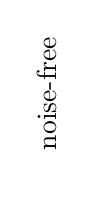
\begin{tikzpicture}
            \node[rotate=90] at (0,0) {noise-free};
            \node at (0,-1.) {~};
    \end{tikzpicture}
    & ~&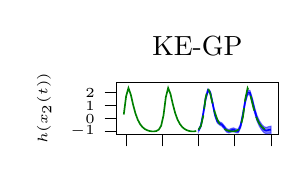
\begin{tikzpicture}
\definecolor{darkgray176}{RGB}{176,176,176}
\definecolor{green}{RGB}{0,128,0}
\definecolor{lightgray204}{RGB}{204,204,204}

\begin{axis}[
    width=.3\textwidth,
    height=.3\textwidth/1.618,
legend cell align={left},
legend style={
  fill opacity=0.8,
  draw opacity=1,
  text opacity=1,
  at={(0.91,0.5)},
  anchor=east,
  draw=lightgray204
},
tick align=outside,
tick pos=left,
title={},
x grid style={darkgray176},
xmin=-1.13387096774194, xmax=1.10161290322581,
yticklabel style = {font = \tiny},
xticklabel style = {font = \tiny},
xtick style={color=black},
y grid style={darkgray176},
ylabel={\tiny $h(x_2(t))$},
ymin=-1.24434151103344, ymax=2.80816290983449,
ytick style={color=black},
title = {KE-GP},
xticklabels={,,}
]
\path [draw=blue, fill=blue, opacity=0.5]
(axis cs:0,-1.02140400442368)
--(axis cs:0,-1.02140400442368)
--(axis cs:0.0322580645161294,-0.652495510938043)
--(axis cs:0.064516129032258,0.262354230312171)
--(axis cs:0.096774193548387,1.38587788384001)
--(axis cs:0.129032258064516,2.07107751409938)
--(axis cs:0.161290322580645,1.91304479941786)
--(axis cs:0.193548387096774,1.096045791632)
--(axis cs:0.225806451612903,0.200357004994826)
--(axis cs:0.258064516129032,-0.326932623751153)
--(axis cs:0.290322580645161,-0.495624209343708)
--(axis cs:0.32258064516129,-0.596688569965196)
--(axis cs:0.354838709677419,-0.808100150089652)
--(axis cs:0.387096774193548,-1.03672170704366)
--(axis cs:0.419354838709678,-1.10878441422885)
--(axis cs:0.451612903225806,-1.03331327373072)
--(axis cs:0.483870967741935,-0.99727272098956)
--(axis cs:0.516129032258065,-1.08882645506894)
--(axis cs:0.548387096774194,-1.10726816024921)
--(axis cs:0.580645161290323,-0.723733555461454)
--(axis cs:0.612903225806452,0.152487838763009)
--(axis cs:0.645161290322581,1.18784215908192)
--(axis cs:0.67741935483871,1.84425611957173)
--(axis cs:0.709677419354839,1.80857170010343)
--(axis cs:0.741935483870968,1.21010470785975)
--(axis cs:0.774193548387097,0.445552659859597)
--(axis cs:0.806451612903226,-0.170389730294337)
--(axis cs:0.838709677419355,-0.582415954342097)
--(axis cs:0.870967741935484,-0.87900913355136)
--(axis cs:0.903225806451613,-1.09089609316336)
--(axis cs:0.935483870967742,-1.16971564012116)
--(axis cs:0.967741935483871,-1.13517934879613)
--(axis cs:1,-1.13540273943964)
--(axis cs:1,-1.13540273943964)
--(axis cs:1,-0.589336779426036)
--(axis cs:0.967741935483871,-0.628004884616578)
--(axis cs:0.935483870967742,-0.685345208139557)
--(axis cs:0.903225806451613,-0.626077562117123)
--(axis cs:0.870967741935484,-0.433322283840301)
--(axis cs:0.838709677419355,-0.154140726890767)
--(axis cs:0.806451612903226,0.241992316668614)
--(axis cs:0.774193548387097,0.840905006264103)
--(axis cs:0.741935483870968,1.58841412615865)
--(axis cs:0.709677419354839,2.17141849752468)
--(axis cs:0.67741935483871,2.19181159353498)
--(axis cs:0.645161290322581,1.52129728516532)
--(axis cs:0.612903225806452,0.472803433036172)
--(axis cs:0.580645161290323,-0.418231775360382)
--(axis cs:0.548387096774194,-0.814981052272685)
--(axis cs:0.516129032258065,-0.805812210943319)
--(axis cs:0.483870967741935,-0.723072183173576)
--(axis cs:0.451612903225806,-0.766537276945688)
--(axis cs:0.419354838709678,-0.846024662513243)
--(axis cs:0.387096774193548,-0.775135242656734)
--(axis cs:0.354838709677419,-0.545246972883508)
--(axis cs:0.32258064516129,-0.337834021537275)
--(axis cs:0.290322580645161,-0.249386944092397)
--(axis cs:0.258064516129032,-0.089932232208076)
--(axis cs:0.225806451612903,0.433451550518775)
--(axis cs:0.193548387096774,1.32119318186608)
--(axis cs:0.161290322580645,2.12897982235537)
--(axis cs:0.129032258064516,2.28022951849028)
--(axis cs:0.096774193548387,1.58874655999785)
--(axis cs:0.064516129032258,0.460734887662643)
--(axis cs:0.0322580645161294,-0.458020404542072)
--(axis cs:0,-0.830871395563078)
--cycle;

\addplot [semithick, blue]
table {%
0 -0.926137699993381
0.0322580645161294 -0.555257957740058
0.064516129032258 0.361544558987407
0.096774193548387 1.48731222191893
0.129032258064516 2.17565351629483
0.161290322580645 2.02101231088661
0.193548387096774 1.20861948674904
0.225806451612903 0.316904277756801
0.258064516129032 -0.208432427979615
0.290322580645161 -0.372505576718053
0.32258064516129 -0.467261295751236
0.354838709677419 -0.67667356148658
0.387096774193548 -0.905928474850199
0.419354838709678 -0.977404538371049
0.451612903225806 -0.899925275338205
0.483870967741935 -0.860172452081568
0.516129032258065 -0.947319333006131
0.548387096774194 -0.961124606260949
0.580645161290323 -0.570982665410918
0.612903225806452 0.312645635899591
0.645161290322581 1.35456972212362
0.67741935483871 2.01803385655336
0.709677419354839 1.98999509881406
0.741935483870968 1.3992594170092
0.774193548387097 0.64322883306185
0.806451612903226 0.0358012931871385
0.838709677419355 -0.368278340616432
0.870967741935484 -0.65616570869583
0.903225806451613 -0.858486827640242
0.935483870967742 -0.92753042413036
0.967741935483871 -0.881592116706355
1 -0.86236975943284
};
\addlegendentry{Prediction}
\addplot [semithick, green]
table {%
-1.03225806451613 0.310677215876974
-1 1.72509317079231
-0.967741935483871 2.35958067123089
-0.935483870967742 1.85373346773129
-0.903225806451613 1.06436987498561
-0.870967741935484 0.39375284056191
-0.838709677419355 -0.0953849947985607
-0.806451612903226 -0.432355212837299
-0.774193548387097 -0.658219795153289
-0.741935483870968 -0.806783922492113
-0.709677419354839 -0.902169203461053
-0.67741935483871 -0.960134910896678
-0.645161290322581 -0.989464930765762
-0.612903225806452 -0.991868128129937
-0.580645161290323 -0.957961550613222
-0.548387096774193 -0.851288713427186
-0.516129032258065 -0.554026202604845
-0.483870967741935 0.243038106393077
-0.451612903225806 1.65036100981229
-0.419354838709677 2.36177948342126
-0.387096774193548 1.89633107767594
-0.354838709677419 1.10719751036095
-0.32258064516129 0.4266122896035
-0.290322580645161 -0.0722737325925517
-0.258064516129032 -0.416693101024244
-0.225806451612903 -0.64782458667783
-0.193548387096774 -0.80001455124028
-0.161290322580645 -0.897905560333097
-0.129032258064516 -0.957683656959815
-0.096774193548387 -0.988507495349605
-0.064516129032258 -0.992535488744642
-0.032258064516129 -0.961254120271588
};
\addlegendentry{Condition}
\addplot [semithick, green, dash pattern=on 5.55pt off 2.4pt]
table {%
0 -0.860613365987377
0.0322580645161294 -0.580085256941532
0.064516129032258 0.177945140645911
0.096774193548387 1.5730115929598
0.129032258064516 2.35986002626562
0.161290322580645 1.93810188327795
0.193548387096774 1.15045548523349
0.225806451612903 0.460068281182399
0.258064516129032 -0.0486707058542165
0.290322580645161 -0.400673957842
0.32258064516129 -0.637181665597286
0.354838709677419 -0.793075190688397
0.387096774193548 -0.893522844289506
0.419354838709678 -0.955142308935798
0.451612903225806 -0.987467578406421
0.483870967741935 -0.993096551558174
0.516129032258065 -0.964343694128448
0.548387096774194 -0.869419253002998
0.580645161290323 -0.604680161786228
0.612903225806452 0.115439309275864
0.645161290322581 1.49344249770474
0.67741935483871 2.3536498063136
0.709677419354839 1.97891203269848
0.741935483870968 1.19411427928786
0.774193548387097 0.494122687936025
0.806451612903226 -0.024568177750323
0.838709677419355 -0.384290661890491
0.870967741935484 -0.626285716196433
0.903225806451613 -0.785962214418609
0.935483870967742 -0.889018792725728
0.967741935483871 -0.952509769733059
1 -0.986345405974012
};
\addlegendentry{Target}
\legend{}
\end{axis}

\end{tikzpicture}

    & 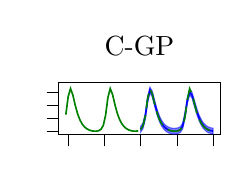
\begin{tikzpicture}
\definecolor{darkgray176}{RGB}{176,176,176}
\definecolor{green}{RGB}{0,128,0}
\definecolor{lightgray204}{RGB}{204,204,204}

\begin{axis}[
    width=.3\textwidth,
    height=.3\textwidth/1.618,
legend cell align={left},
legend style={
  fill opacity=0.8,
  draw opacity=1,
  text opacity=1,
  at={(0.91,0.5)},
  anchor=east,
  draw=lightgray204
},
tick align=outside,
tick pos=left,
title={},
x grid style={darkgray176},
xmin=-1.13387096774194, xmax=1.10161290322581,
yticklabel style = {font = \tiny},
xticklabel style = {font = \tiny},
xtick style={color=black},
y grid style={darkgray176},
yticklabels={,,},
ymin=-1.24434151103344, ymax=2.80816290983449,
ytick style={color=black},
title = {C-GP},
xticklabels={,,}
]
\path [draw=blue, fill=blue, opacity=0.5]
(axis cs:0,-1.05108515937071)
--(axis cs:0,-1.05108515937071)
--(axis cs:0.0322580645161294,-0.793160590795055)
--(axis cs:0.064516129032258,-0.0603062917985711)
--(axis cs:0.096774193548387,1.22882234949531)
--(axis cs:0.129032258064516,1.98426786044561)
--(axis cs:0.161290322580645,1.66841311569064)
--(axis cs:0.193548387096774,0.958310780161869)
--(axis cs:0.225806451612903,0.306394904418292)
--(axis cs:0.258064516129032,-0.212888207688193)
--(axis cs:0.290322580645161,-0.582703101588369)
--(axis cs:0.32258064516129,-0.835874367322634)
--(axis cs:0.354838709677419,-1.00203768354496)
--(axis cs:0.387096774193548,-1.10714748485308)
--(axis cs:0.419354838709678,-1.17140308919753)
--(axis cs:0.451612903225806,-1.19965554864374)
--(axis cs:0.483870967741935,-1.19530653556042)
--(axis cs:0.516129032258065,-1.15936290453452)
--(axis cs:0.548387096774194,-1.0803418364458)
--(axis cs:0.580645161290323,-0.800198044363484)
--(axis cs:0.612903225806452,0.00716944377067719)
--(axis cs:0.645161290322581,1.16755075412088)
--(axis cs:0.67741935483871,1.8172387957578)
--(axis cs:0.709677419354839,1.58508429550798)
--(axis cs:0.741935483870968,0.974585357927645)
--(axis cs:0.774193548387097,0.357310713603246)
--(axis cs:0.806451612903226,-0.15783710235564)
--(axis cs:0.838709677419355,-0.531319888487658)
--(axis cs:0.870967741935484,-0.798065930451727)
--(axis cs:0.903225806451613,-0.97783090509574)
--(axis cs:0.935483870967742,-1.09261986576696)
--(axis cs:0.967741935483871,-1.15862392448967)
--(axis cs:1,-1.18635885172024)
--(axis cs:1,-1.18635885172024)
--(axis cs:1,-0.741559354342373)
--(axis cs:0.967741935483871,-0.713829125691939)
--(axis cs:0.935483870967742,-0.647831583308663)
--(axis cs:0.903225806451613,-0.533053684862027)
--(axis cs:0.870967741935484,-0.353302013267092)
--(axis cs:0.838709677419355,-0.0865646795851854)
--(axis cs:0.806451612903226,0.286913791961969)
--(axis cs:0.774193548387097,0.802061551717969)
--(axis cs:0.741935483870968,1.41933709365362)
--(axis cs:0.709677419354839,2.0298323542427)
--(axis cs:0.67741935483871,2.26198510247366)
--(axis cs:0.645161290322581,1.61229702312937)
--(axis cs:0.612903225806452,0.45191606222082)
--(axis cs:0.580645161290323,-0.355451984459446)
--(axis cs:0.548387096774194,-0.635596974629444)
--(axis cs:0.516129032258065,-0.714619200204716)
--(axis cs:0.483870967741935,-0.750562600662023)
--(axis cs:0.451612903225806,-0.754910083090394)
--(axis cs:0.419354838709678,-0.726655065900912)
--(axis cs:0.387096774193548,-0.662396999060331)
--(axis cs:0.354838709677419,-0.557290313339431)
--(axis cs:0.32258064516129,-0.391130080617812)
--(axis cs:0.290322580645161,-0.137956495689864)
--(axis cs:0.258064516129032,0.231857750074283)
--(axis cs:0.225806451612903,0.751141053470489)
--(axis cs:0.193548387096774,1.40305874079444)
--(axis cs:0.161290322580645,2.11316494792416)
--(axis cs:0.129032258064516,2.4290291703633)
--(axis cs:0.096774193548387,1.6735944055097)
--(axis cs:0.064516129032258,0.384476746922106)
--(axis cs:0.0322580645161294,-0.348367611066797)
--(axis cs:0,-0.606285059749114)
--cycle;

\addplot [semithick, blue]
table {%
0 -0.828685109559914
0.0322580645161294 -0.570764100930926
0.064516129032258 0.162085227561768
0.096774193548387 1.4512083775025
0.129032258064516 2.20664851540445
0.161290322580645 1.8907890318074
0.193548387096774 1.18068476047816
0.225806451612903 0.528767978944391
0.258064516129032 0.00948477119304473
0.290322580645161 -0.360329798639116
0.32258064516129 -0.613502223970223
0.354838709677419 -0.779663998442196
0.387096774193548 -0.884772241956707
0.419354838709678 -0.94902907754922
0.451612903225806 -0.977282815867066
0.483870967741935 -0.972934568111222
0.516129032258065 -0.93699105236962
0.548387096774194 -0.857969405537623
0.580645161290323 -0.577825014411465
0.612903225806452 0.229542752995749
0.645161290322581 1.38992388862513
0.67741935483871 2.03961194911573
0.709677419354839 1.80745832487534
0.741935483870968 1.19696122579063
0.774193548387097 0.579686132660608
0.806451612903226 0.0645383448031647
0.838709677419355 -0.308942284036422
0.870967741935484 -0.57568397185941
0.903225806451613 -0.755442294978883
0.935483870967742 -0.87022572453781
0.967741935483871 -0.936226525090803
1 -0.963959103031306
};
\addlegendentry{Prediction}
\addplot [semithick, green]
table {%
-1.03225806451613 0.303603707030286
-1 1.69110343786114
-0.967741935483871 2.31351669120059
-0.935483870967742 1.81729572009365
-0.903225806451613 1.04295365427054
-0.870967741935484 0.385098409128619
-0.838709677419355 -0.0947311717972172
-0.806451612903226 -0.425288873159369
-0.774193548387097 -0.646855270285042
-0.741935483870968 -0.792592233996031
-0.709677419354839 -0.886162340589994
-0.67741935483871 -0.94302496518416
-0.645161290322581 -0.971796837088032
-0.612903225806452 -0.974154301795878
-0.580645161290323 -0.940892963775511
-0.548387096774193 -0.836250102269154
-0.516129032258065 -0.54464447358633
-0.483870967741935 0.237251764466004
-0.451612903225806 1.61779342401137
-0.419354838709677 2.31567366016837
-0.387096774193548 1.85908270088021
-0.354838709677419 1.08496628312198
-0.32258064516129 0.417332545446167
-0.290322580645161 -0.0720597150884879
-0.258064516129032 -0.409924810099038
-0.225806451612903 -0.636657881807129
-0.193548387096774 -0.785951683345303
-0.161290322580645 -0.881979834254542
-0.129032258064516 -0.940620358416416
-0.096774193548387 -0.970857621592344
-0.064516129032258 -0.974808962590712
-0.032258064516129 -0.944122876092924
};
\addlegendentry{Condition}
\addplot [semithick, green, dash pattern=on 5.55pt off 2.4pt]
table {%
0 -0.845397307426445
0.0322580645161294 -0.570207626173946
0.064516129032258 0.173397512723927
0.096774193548387 1.54191596046199
0.129032258064516 2.31379073013104
0.161290322580645 1.90005861134556
0.193548387096774 1.12740106214391
0.225806451612903 0.450151872143582
0.258064516129032 -0.0489058520877034
0.290322580645161 -0.394210509948319
0.32258064516129 -0.626217494675471
0.354838709677419 -0.779144378277501
0.387096774193548 -0.877680520951649
0.419354838709678 -0.938127372044891
0.451612903225806 -0.969837494186583
0.483870967741935 -0.975359348423147
0.516129032258065 -0.947153655602924
0.548387096774194 -0.854035619106571
0.580645161290323 -0.594334491918945
0.612903225806452 0.112081162395787
0.645161290322581 1.463861058815
0.67741935483871 2.30769869017498
0.709677419354839 1.94009214684081
0.741935483870968 1.17022903279026
0.774193548387097 0.483558226222138
0.806451612903226 -0.0252619931929575
0.838709677419355 -0.378138986826819
0.870967741935484 -0.615528894332488
0.903225806451613 -0.772166761385214
0.935483870967742 -0.873262181133951
0.967741935483871 -0.935544929855583
1 -0.968736676607071
};
\addlegendentry{Target}
\legend{}
\end{axis}

\end{tikzpicture}

    &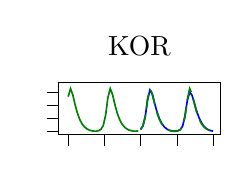
\begin{tikzpicture}
\definecolor{darkgray176}{RGB}{176,176,176}
\definecolor{green}{RGB}{0,128,0}
\definecolor{lightgray204}{RGB}{204,204,204}

\begin{axis}[
    width=.3\textwidth,
    height=.3\textwidth/1.618,
legend cell align={left},
legend style={
  fill opacity=0.8,
  draw opacity=1,
  text opacity=1,
  at={(0.91,0.5)},
  anchor=east,
  draw=lightgray204
},
tick align=outside,
tick pos=left,
title={},
x grid style={darkgray176},
xmin=-1.13387096774194, xmax=1.10161290322581,
yticklabel style = {font = \tiny},
xticklabel style = {font = \tiny},
xtick style={color=black},
y grid style={darkgray176},
ymin=-1.24434151103344, ymax=2.80816290983449,
ytick style={color=black},
yticklabels={,,},
title = {KOR},
xticklabels={,,}
]
\addplot [semithick, blue]
table {%
0 -0.828685109559914
0.0322580645161294 -0.570764100930926
0.064516129032258 0.162085227561768
0.096774193548387 1.4512083775025
0.129032258064516 2.20664851540445
0.161290322580645 1.8907890318074
0.193548387096774 1.18068476047816
0.225806451612903 0.528767978944391
0.258064516129032 0.00948477119304473
0.290322580645161 -0.360329798639116
0.32258064516129 -0.613502223970223
0.354838709677419 -0.779663998442196
0.387096774193548 -0.884772241956707
0.419354838709678 -0.94902907754922
0.451612903225806 -0.977282815867066
0.483870967741935 -0.972934568111222
0.516129032258065 -0.93699105236962
0.548387096774194 -0.857969405537623
0.580645161290323 -0.577825014411465
0.612903225806452 0.229542752995749
0.645161290322581 1.38992388862513
0.67741935483871 2.03961194911573
0.709677419354839 1.80745832487534
0.741935483870968 1.19696122579063
0.774193548387097 0.579686132660608
0.806451612903226 0.0645383448031647
0.838709677419355 -0.308942284036422
0.870967741935484 -0.57568397185941
0.903225806451613 -0.755442294978883
0.935483870967742 -0.87022572453781
0.967741935483871 -0.936226525090803
1 -0.963959103031306
};
\addlegendentry{Prediction}
\addplot [semithick, green]
table {%
-1 1.69110343786114
-0.967741935483871 2.31351669120059
-0.935483870967742 1.81729572009365
-0.903225806451613 1.04295365427054
-0.870967741935484 0.385098409128619
-0.838709677419355 -0.0947311717972172
-0.806451612903226 -0.425288873159369
-0.774193548387097 -0.646855270285042
-0.741935483870968 -0.792592233996031
-0.709677419354839 -0.886162340589994
-0.67741935483871 -0.94302496518416
-0.645161290322581 -0.971796837088032
-0.612903225806452 -0.974154301795878
-0.580645161290323 -0.940892963775511
-0.548387096774193 -0.836250102269154
-0.516129032258065 -0.54464447358633
-0.483870967741935 0.237251764466004
-0.451612903225806 1.61779342401137
-0.419354838709677 2.31567366016837
-0.387096774193548 1.85908270088021
-0.354838709677419 1.08496628312198
-0.32258064516129 0.417332545446167
-0.290322580645161 -0.0720597150884879
-0.258064516129032 -0.409924810099038
-0.225806451612903 -0.636657881807129
-0.193548387096774 -0.785951683345303
-0.161290322580645 -0.881979834254542
-0.129032258064516 -0.940620358416416
-0.096774193548387 -0.970857621592344
-0.064516129032258 -0.974808962590712
-0.032258064516129 -0.944122876092924
};
\addlegendentry{Condition}
\addplot [semithick, green, dash pattern=on 5.55pt off 2.4pt]
table {%
0 -0.845397307426445
0.0322580645161294 -0.570207626173946
0.064516129032258 0.173397512723927
0.096774193548387 1.54191596046199
0.129032258064516 2.31379073013104
0.161290322580645 1.90005861134556
0.193548387096774 1.12740106214391
0.225806451612903 0.450151872143582
0.258064516129032 -0.0489058520877034
0.290322580645161 -0.394210509948319
0.32258064516129 -0.626217494675471
0.354838709677419 -0.779144378277501
0.387096774193548 -0.877680520951649
0.419354838709678 -0.938127372044891
0.451612903225806 -0.969837494186583
0.483870967741935 -0.975359348423147
0.516129032258065 -0.947153655602924
0.548387096774194 -0.854035619106571
0.580645161290323 -0.594334491918945
0.612903225806452 0.112081162395787
0.645161290322581 1.463861058815
0.67741935483871 2.30769869017498
0.709677419354839 1.94009214684081
0.741935483870968 1.17022903279026
0.774193548387097 0.483558226222138
0.806451612903226 -0.0252619931929575
0.838709677419355 -0.378138986826819
0.870967741935484 -0.615528894332488
0.903225806451613 -0.772166761385214
0.935483870967742 -0.873262181133951
0.967741935483871 -0.935544929855583
1 -0.968736676607071
};
\addlegendentry{Target}
\legend{}
\end{axis}

\end{tikzpicture}

    &\definecolor{fig_green}{RGB}{0,128,0}
    \begin{tikzpicture}
        \node at (0,0) {\begin{tikzpicture} 
    \begin{axis}[%
    hide axis,
    xmin=10,
    xmax=50,
    ymin=0,
    ymax=0.4,
    legend style={draw=white!15!black,legend cell align=left}
    ]
    \addlegendimage{semithick, fig_green}
    \addlegendentry{\tiny input};
    \addlegendimage{semithick, fig_green, dash pattern=on 5.55pt off 2.4pt}
    \addlegendentry{\tiny ground truth};
    \addlegendimage{semithick, blue};
    \addlegendentry{\tiny prediction};
    \end{axis}
\end{tikzpicture}};
    \node at (0,-1.) {~};
    \end{tikzpicture}
    \\
    \begin{tikzpicture}
            \node[rotate=90] at (0,0) {noisy};
            \node at (0,-1.65) {~};
    \end{tikzpicture}    
    &~ &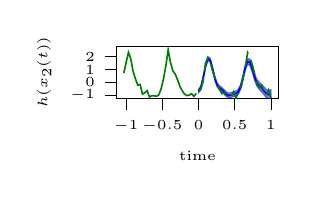
\begin{tikzpicture}
\definecolor{darkgray176}{RGB}{176,176,176}
\definecolor{green}{RGB}{0,128,0}
\definecolor{lightgray204}{RGB}{204,204,204}

\begin{axis}[
    width=.3\textwidth,
    height=.3\textwidth/1.618,
legend cell align={left},
legend style={
  fill opacity=0.8,
  draw opacity=1,
  text opacity=1,
  at={(0.91,0.5)},
  anchor=east,
  draw=lightgray204
},
tick align=outside,
tick pos=left,
title={},
x grid style={darkgray176},
xlabel={\tiny time},
xmin=-1.13387096774194, xmax=1.10161290322581,
yticklabel style = {font = \tiny},
xticklabel style = {font = \tiny},
xtick style={color=black},
y grid style={darkgray176},
ylabel={\tiny $h(x_2(t))$},
ymin=-1.24434151103344, ymax=2.80816290983449,
ytick style={color=black}
]
\path [draw=blue, fill=blue, opacity=0.5]
(axis cs:0,-0.791884136999424)
--(axis cs:0,-0.791884136999424)
--(axis cs:0.0322580645161294,-0.532216532304019)
--(axis cs:0.064516129032258,0.207228559293209)
--(axis cs:0.096774193548387,1.12442474773327)
--(axis cs:0.129032258064516,1.68552099965311)
--(axis cs:0.161290322580645,1.56756057868288)
--(axis cs:0.193548387096774,0.908504125338844)
--(axis cs:0.225806451612903,0.146043870272565)
--(axis cs:0.258064516129032,-0.366882740438619)
--(axis cs:0.290322580645161,-0.596461580106275)
--(axis cs:0.32258064516129,-0.730623805831874)
--(axis cs:0.354838709677419,-0.913165271816812)
--(axis cs:0.387096774193548,-1.10654589884703)
--(axis cs:0.419354838709678,-1.19381854020165)
--(axis cs:0.451612903225806,-1.1546485659785)
--(axis cs:0.483870967741935,-1.08630398785724)
--(axis cs:0.516129032258065,-1.04849802441944)
--(axis cs:0.548387096774194,-0.935844580875931)
--(axis cs:0.580645161290323,-0.556390585828836)
--(axis cs:0.612903225806452,0.13874292125789)
--(axis cs:0.645161290322581,0.915902956607306)
--(axis cs:0.67741935483871,1.38730562268057)
--(axis cs:0.709677419354839,1.31274347655288)
--(axis cs:0.741935483870968,0.790708060720758)
--(axis cs:0.774193548387097,0.158464904288433)
--(axis cs:0.806451612903226,-0.298006792955262)
--(axis cs:0.838709677419355,-0.542627672001628)
--(axis cs:0.870967741935484,-0.721536980353704)
--(axis cs:0.903225806451613,-0.942388520552518)
--(axis cs:0.935483870967742,-1.15803749659711)
--(axis cs:0.967741935483871,-1.26309387894733)
--(axis cs:1,-1.24564270290988)
--(axis cs:1,-1.24564270290988)
--(axis cs:1,-0.553480274017001)
--(axis cs:0.967741935483871,-0.609085413130824)
--(axis cs:0.935483870967742,-0.531751521780701)
--(axis cs:0.903225806451613,-0.338120947030914)
--(axis cs:0.870967741935484,-0.137210070592655)
--(axis cs:0.838709677419355,0.0221297258593717)
--(axis cs:0.806451612903226,0.24789628860997)
--(axis cs:0.774193548387097,0.68638603957788)
--(axis cs:0.741935483870968,1.30113999406795)
--(axis cs:0.709677419354839,1.80656027208635)
--(axis cs:0.67741935483871,1.86440299114285)
--(axis cs:0.645161290322581,1.37557834692631)
--(axis cs:0.612903225806452,0.581761298262494)
--(axis cs:0.580645161290323,-0.128417100507951)
--(axis cs:0.548387096774194,-0.52080342500663)
--(axis cs:0.516129032258065,-0.644678468860948)
--(axis cs:0.483870967741935,-0.693848595375854)
--(axis cs:0.451612903225806,-0.773011108705527)
--(axis cs:0.419354838709678,-0.8207407389894)
--(axis cs:0.387096774193548,-0.740992616247295)
--(axis cs:0.354838709677419,-0.555241944757114)
--(axis cs:0.32258064516129,-0.380263917490026)
--(axis cs:0.290322580645161,-0.253998834224472)
--(axis cs:0.258064516129032,-0.0324742077203883)
--(axis cs:0.225806451612903,0.47322937545827)
--(axis cs:0.193548387096774,1.22944838870588)
--(axis cs:0.161290322580645,1.88216516482222)
--(axis cs:0.129032258064516,1.99311527479243)
--(axis cs:0.096774193548387,1.42551734614703)
--(axis cs:0.064516129032258,0.501904359793165)
--(axis cs:0.0322580645161294,-0.245188439871079)
--(axis cs:0,-0.509073434700109)
--cycle;

\addplot [semithick, blue]
table {%
0 -0.650478785849767
0.0322580645161294 -0.388702486087549
0.064516129032258 0.354566459543187
0.096774193548387 1.27497104694015
0.129032258064516 1.83931813722277
0.161290322580645 1.72486287175255
0.193548387096774 1.06897625702236
0.225806451612903 0.309636622865418
0.258064516129032 -0.199678474079504
0.290322580645161 -0.425230207165373
0.32258064516129 -0.55544386166095
0.354838709677419 -0.734203608286963
0.387096774193548 -0.923769257547163
0.419354838709678 -1.00727963959552
0.451612903225806 -0.963829837342014
0.483870967741935 -0.890076291616549
0.516129032258065 -0.846588246640194
0.548387096774194 -0.728324002941281
0.580645161290323 -0.342403843168393
0.612903225806452 0.360252109760192
0.645161290322581 1.14574065176681
0.67741935483871 1.62585430691171
0.709677419354839 1.55965187431961
0.741935483870968 1.04592402739435
0.774193548387097 0.422425471933156
0.806451612903226 -0.0250552521726459
0.838709677419355 -0.260248973071128
0.870967741935484 -0.42937352547318
0.903225806451613 -0.640254733791716
0.935483870967742 -0.844894509188906
0.967741935483871 -0.936089646039077
1 -0.899561488463438
};
\addlegendentry{Prediction}
\addplot [semithick, green]
table {%
-1.03225806451613 0.729314096916195
-1 1.5430002430531
-0.967741935483871 2.32204403870171
-0.935483870967742 1.831985798904
-0.903225806451613 0.851433703296098
-0.870967741935484 0.279354081877078
-0.838709677419355 -0.210590170919282
-0.806451612903226 -0.154089766822581
-0.774193548387097 -0.89795080770656
-0.741935483870968 -0.788817886111994
-0.709677419354839 -0.631217039088834
-0.67741935483871 -1.11565489128188
-0.645161290322581 -1.0186823441863
-0.612903225806452 -1.02455755343605
-0.580645161290323 -1.06131914172655
-0.548387096774193 -0.952046399419613
-0.516129032258065 -0.466246020590151
-0.483870967741935 0.262503198938305
-0.451612903225806 1.29173786310598
-0.419354838709677 2.51920556711464
-0.387096774193548 1.54711284138206
-0.354838709677419 0.915038117881071
-0.32258064516129 0.656212982887232
-0.290322580645161 0.221915856154588
-0.258064516129032 -0.281944627110773
-0.225806451612903 -0.633593952285014
-0.193548387096774 -0.895240317440411
-0.161290322580645 -1.00560588014814
-0.129032258064516 -0.974031437037782
-0.096774193548387 -0.866150101663904
-0.064516129032258 -1.07102836219983
-0.032258064516129 -0.835479545663183
};
\addlegendentry{Condition}
\addplot [semithick, green, dash pattern=on 5.55pt off 2.4pt]
table {%
0 -0.739654414051487
0.0322580645161294 -0.518329938112951
0.064516129032258 0.116995492630876
0.096774193548387 1.4830385503286
0.129032258064516 1.92918851810535
0.161290322580645 1.60484919087504
0.193548387096774 0.902948829211309
0.225806451612903 0.360083074779615
0.258064516129032 0.038407028127166
0.290322580645161 -0.535312914336627
0.32258064516129 -0.850668308618081
0.354838709677419 -0.773023157271037
0.387096774193548 -1.12963704153207
0.419354838709678 -1.06214760780795
0.451612903225806 -1.04132234674408
0.483870967741935 -0.728286752014149
0.516129032258065 -1.19049036317343
0.548387096774194 -0.786213082699808
0.580645161290323 -0.567579376473479
0.612903225806452 0.335513082155103
0.645161290322581 1.1374733999599
0.67741935483871 2.30787657939374
0.709677419354839 1.96813566944444
0.741935483870968 1.36715134974877
0.774193548387097 0.675192568868016
0.806451612903226 -0.179955450959619
0.838709677419355 -0.372618434067805
0.870967741935484 -0.210140874568701
0.903225806451613 -0.699218180799252
0.935483870967742 -0.996483428586153
0.967741935483871 -0.577931038414108
1 -1.19679478002127
};
\addlegendentry{Target}
\legend{}
\end{axis}

\end{tikzpicture}

    & 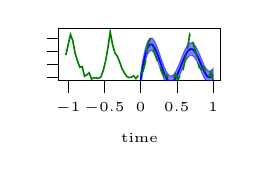
\begin{tikzpicture}
\definecolor{darkgray176}{RGB}{176,176,176}
\definecolor{green}{RGB}{0,128,0}
\definecolor{lightgray204}{RGB}{204,204,204}

\begin{axis}[
    width=.3\textwidth,
    height=.3\textwidth/1.618,
legend cell align={left},
legend style={
  fill opacity=0.8,
  draw opacity=1,
  text opacity=1,
  at={(0.91,0.5)},
  anchor=east,
  draw=lightgray204
},
tick align=outside,
tick pos=left,
title={},
x grid style={darkgray176},
xlabel={\tiny time},
xmin=-1.13387096774194, xmax=1.10161290322581,
yticklabel style = {font = \tiny},
xticklabel style = {font = \tiny},
xtick style={color=black},
y grid style={darkgray176},
ymin=-1.24434151103344, ymax=2.80816290983449,
ytick style={color=black},
yticklabels={,,},
]
\path [draw=blue, fill=blue, opacity=0.5]
(axis cs:0,-1.665446045318)
--(axis cs:0,-1.665446045318)
--(axis cs:0.0322580645161294,-0.568897619418134)
--(axis cs:0.064516129032258,0.263031758801038)
--(axis cs:0.096774193548387,0.80837881476712)
--(axis cs:0.129032258064516,1.06689859178334)
--(axis cs:0.161290322580645,1.05987425552174)
--(axis cs:0.193548387096774,0.827975353710028)
--(axis cs:0.225806451612903,0.427391510412111)
--(axis cs:0.258064516129032,-0.0753940214809364)
--(axis cs:0.290322580645161,-0.609730884208127)
--(axis cs:0.32258064516129,-1.10730328548885)
--(axis cs:0.354838709677419,-1.50844223065865)
--(axis cs:0.387096774193548,-1.76767234362311)
--(axis cs:0.419354838709678,-1.85794397149951)
--(axis cs:0.451612903225806,-1.77307757287024)
--(axis cs:0.483870967741935,-1.52808132186236)
--(axis cs:0.516129032258065,-1.15719445331029)
--(axis cs:0.548387096774194,-0.709747383335965)
--(axis cs:0.580645161290323,-0.244192486820868)
--(axis cs:0.612903225806452,0.179086613560679)
--(axis cs:0.645161290322581,0.505374216416193)
--(axis cs:0.67741935483871,0.692700794731376)
--(axis cs:0.709677419354839,0.717475249796781)
--(axis cs:0.741935483870968,0.577886228992258)
--(axis cs:0.774193548387097,0.294555925632589)
--(axis cs:0.806451612903226,-0.0917064341730509)
--(axis cs:0.838709677419355,-0.52479970843623)
--(axis cs:0.870967741935484,-0.940245125827395)
--(axis cs:0.903225806451613,-1.27320560445854)
--(axis cs:0.935483870967742,-1.46655351593068)
--(axis cs:0.967741935483871,-1.47794982792781)
--(axis cs:1,-1.28506461143995)
--(axis cs:1,-1.28506461143995)
--(axis cs:1,-0.308494704515844)
--(axis cs:0.967741935483871,-0.502960017690905)
--(axis cs:0.935483870967742,-0.491970746399289)
--(axis cs:0.903225806451613,-0.298729000184287)
--(axis cs:0.870967741935484,0.03416669025934)
--(axis cs:0.838709677419355,0.449555573601588)
--(axis cs:0.806451612903226,0.882610046978934)
--(axis cs:0.774193548387097,1.26885004869444)
--(axis cs:0.741935483870968,1.55216499587092)
--(axis cs:0.709677419354839,1.69173937657283)
--(axis cs:0.67741935483871,1.66695089356827)
--(axis cs:0.645161290322581,1.47961336153512)
--(axis cs:0.612903225806452,1.15331907153329)
--(axis cs:0.580645161290323,0.730036686685325)
--(axis cs:0.548387096774194,0.264480380521523)
--(axis cs:0.516129032258065,-0.182967136242761)
--(axis cs:0.483870967741935,-0.553853726218446)
--(axis cs:0.451612903225806,-0.798849088776305)
--(axis cs:0.419354838709678,-0.883714042924335)
--(axis cs:0.387096774193548,-0.79343981256301)
--(axis cs:0.354838709677419,-0.53420442976094)
--(axis cs:0.32258064516129,-0.133056136115851)
--(axis cs:0.290322580645161,0.364529431938274)
--(axis cs:0.258064516129032,0.898881466603521)
--(axis cs:0.225806451612903,1.40168402321776)
--(axis cs:0.193548387096774,1.80229195788188)
--(axis cs:0.161290322580645,2.03423047083746)
--(axis cs:0.129032258064516,2.04131128161313)
--(axis cs:0.096774193548387,1.78285641240048)
--(axis cs:0.064516129032258,1.23761649151677)
--(axis cs:0.0322580645161294,0.406094571417332)
--(axis cs:0,-0.68887762798297)
--cycle;

\addplot [semithick, blue]
table {%
0 -1.17716183665049
0.0322580645161294 -0.0814015240004009
0.064516129032258 0.750324125158903
0.096774193548387 1.2956176135838
0.129032258064516 1.55410493669824
0.161290322580645 1.5470523631796
0.193548387096774 1.31513365579596
0.225806451612903 0.914537766814935
0.258064516129032 0.411743722561292
0.290322580645161 -0.122600726134926
0.32258064516129 -0.620179710802348
0.354838709677419 -1.02132333020979
0.387096774193548 -1.28055607809306
0.419354838709678 -1.37082900721192
0.451612903225806 -1.28596333082327
0.483870967741935 -1.0409675240404
0.516129032258065 -0.670080794776524
0.548387096774194 -0.222633501407221
0.580645161290323 0.242922099932229
0.612903225806452 0.666202842546984
0.645161290322581 0.992493788975658
0.67741935483871 1.17982584414982
0.709677419354839 1.2046073131848
0.741935483870968 1.06502561243159
0.774193548387097 0.781702987163514
0.806451612903226 0.395451806402942
0.838709677419355 -0.0376220674173207
0.870967741935484 -0.453039217784028
0.903225806451613 -0.785967302321414
0.935483870967742 -0.979262131164983
0.967741935483871 -0.990454922809359
1 -0.796779657977895
};
\addlegendentry{Prediction}
\addplot [semithick, green]
table {%
-1.03225806451613 0.729314096916195
-1 1.5430002430531
-0.967741935483871 2.32204403870171
-0.935483870967742 1.831985798904
-0.903225806451613 0.851433703296098
-0.870967741935484 0.279354081877078
-0.838709677419355 -0.210590170919282
-0.806451612903226 -0.154089766822581
-0.774193548387097 -0.89795080770656
-0.741935483870968 -0.788817886111994
-0.709677419354839 -0.631217039088834
-0.67741935483871 -1.11565489128188
-0.645161290322581 -1.0186823441863
-0.612903225806452 -1.02455755343605
-0.580645161290323 -1.06131914172655
-0.548387096774193 -0.952046399419613
-0.516129032258065 -0.466246020590151
-0.483870967741935 0.262503198938305
-0.451612903225806 1.29173786310598
-0.419354838709677 2.51920556711464
-0.387096774193548 1.54711284138206
-0.354838709677419 0.915038117881071
-0.32258064516129 0.656212982887232
-0.290322580645161 0.221915856154588
-0.258064516129032 -0.281944627110773
-0.225806451612903 -0.633593952285014
-0.193548387096774 -0.895240317440411
-0.161290322580645 -1.00560588014814
-0.129032258064516 -0.974031437037782
-0.096774193548387 -0.866150101663904
-0.064516129032258 -1.07102836219983
-0.032258064516129 -0.835479545663183
};
\addlegendentry{Condition}
\addplot [semithick, green, dash pattern=on 5.55pt off 2.4pt]
table {%
0 -0.739654414051487
0.0322580645161294 -0.518329938112951
0.064516129032258 0.116995492630876
0.096774193548387 1.4830385503286
0.129032258064516 1.92918851810535
0.161290322580645 1.60484919087504
0.193548387096774 0.902948829211309
0.225806451612903 0.360083074779615
0.258064516129032 0.038407028127166
0.290322580645161 -0.535312914336627
0.32258064516129 -0.850668308618081
0.354838709677419 -0.773023157271037
0.387096774193548 -1.12963704153207
0.419354838709678 -1.06214760780795
0.451612903225806 -1.04132234674408
0.483870967741935 -0.728286752014149
0.516129032258065 -1.19049036317343
0.548387096774194 -0.786213082699808
0.580645161290323 -0.567579376473479
0.612903225806452 0.335513082155103
0.645161290322581 1.1374733999599
0.67741935483871 2.30787657939374
0.709677419354839 1.96813566944444
0.741935483870968 1.36715134974877
0.774193548387097 0.675192568868016
0.806451612903226 -0.179955450959619
0.838709677419355 -0.372618434067805
0.870967741935484 -0.210140874568701
0.903225806451613 -0.699218180799252
0.935483870967742 -0.996483428586153
0.967741935483871 -0.577931038414108
1 -1.19679478002127
};
\addlegendentry{Target}
\legend{}
\end{axis}

\end{tikzpicture}

    &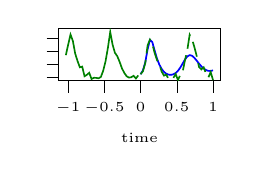
\begin{tikzpicture}
\definecolor{darkgray176}{RGB}{176,176,176}
\definecolor{green}{RGB}{0,128,0}
\definecolor{lightgray204}{RGB}{204,204,204}

\begin{axis}[
    width=.3\textwidth,
    height=.3\textwidth/1.618,
legend cell align={left},
legend style={
  fill opacity=0.8,
  draw opacity=1,
  text opacity=1,
  at={(0.91,0.5)},
  anchor=east,
  draw=lightgray204
},
tick align=outside,
tick pos=left,
title={},
x grid style={darkgray176},
xlabel={\tiny time},
xmin=-1.13387096774194, xmax=1.10161290322581,
yticklabel style = {font = \tiny},
xticklabel style = {font = \tiny},
xtick style={color=black},
y grid style={darkgray176},
ymin=-1.24434151103344, ymax=2.80816290983449,
ytick style={color=black},
yticklabels={,,},
]
\path [draw=blue, fill=blue, opacity=0.5]
(axis cs:0,-0.739898853705199)
--(axis cs:0,-0.739898853705199)
--(axis cs:0.0322580645161294,-0.442945945873865)
--(axis cs:0.064516129032258,0.177347417694429)
--(axis cs:0.096774193548387,1.1793753362096)
--(axis cs:0.129032258064516,1.9082301566808)
--(axis cs:0.161290322580645,1.74112809427527)
--(axis cs:0.193548387096774,1.0935983658069)
--(axis cs:0.225806451612903,0.475966804677645)
--(axis cs:0.258064516129032,0.00745292875602004)
--(axis cs:0.290322580645161,-0.330334796939457)
--(axis cs:0.32258064516129,-0.563439462459379)
--(axis cs:0.354838709677419,-0.705507882191618)
--(axis cs:0.387096774193548,-0.775254931041344)
--(axis cs:0.419354838709678,-0.789205189430896)
--(axis cs:0.451612903225806,-0.750487798384455)
--(axis cs:0.483870967741935,-0.651092336115223)
--(axis cs:0.516129032258065,-0.478710653656521)
--(axis cs:0.548387096774194,-0.227412542331311)
--(axis cs:0.580645161290323,0.083543012528116)
--(axis cs:0.612903225806452,0.395990468795268)
--(axis cs:0.645161290322581,0.630876528174991)
--(axis cs:0.67741935483871,0.730448613899942)
--(axis cs:0.709677419354839,0.685308374337714)
--(axis cs:0.741935483870968,0.528205912488009)
--(axis cs:0.774193548387097,0.309887456428381)
--(axis cs:0.806451612903226,0.0779767485881812)
--(axis cs:0.838709677419355,-0.132959994201391)
--(axis cs:0.870967741935484,-0.302395337257076)
--(axis cs:0.903225806451613,-0.4204759409994)
--(axis cs:0.935483870967742,-0.483716978187525)
--(axis cs:0.967741935483871,-0.491757964036874)
--(axis cs:1,-0.446135940069033)
--(axis cs:1,-0.446135940069033)
--(axis cs:1,-0.446135940069033)
--(axis cs:0.967741935483871,-0.491757964036874)
--(axis cs:0.935483870967742,-0.483716978187525)
--(axis cs:0.903225806451613,-0.4204759409994)
--(axis cs:0.870967741935484,-0.302395337257076)
--(axis cs:0.838709677419355,-0.132959994201391)
--(axis cs:0.806451612903226,0.0779767485881812)
--(axis cs:0.774193548387097,0.309887456428381)
--(axis cs:0.741935483870968,0.528205912488009)
--(axis cs:0.709677419354839,0.685308374337714)
--(axis cs:0.67741935483871,0.730448613899942)
--(axis cs:0.645161290322581,0.630876528174991)
--(axis cs:0.612903225806452,0.395990468795268)
--(axis cs:0.580645161290323,0.083543012528116)
--(axis cs:0.548387096774194,-0.227412542331311)
--(axis cs:0.516129032258065,-0.478710653656521)
--(axis cs:0.483870967741935,-0.651092336115223)
--(axis cs:0.451612903225806,-0.750487798384455)
--(axis cs:0.419354838709678,-0.789205189430896)
--(axis cs:0.387096774193548,-0.775254931041344)
--(axis cs:0.354838709677419,-0.705507882191618)
--(axis cs:0.32258064516129,-0.563439462459379)
--(axis cs:0.290322580645161,-0.330334796939457)
--(axis cs:0.258064516129032,0.00745292875602004)
--(axis cs:0.225806451612903,0.475966804677645)
--(axis cs:0.193548387096774,1.0935983658069)
--(axis cs:0.161290322580645,1.74112809427527)
--(axis cs:0.129032258064516,1.9082301566808)
--(axis cs:0.096774193548387,1.1793753362096)
--(axis cs:0.064516129032258,0.177347417694429)
--(axis cs:0.0322580645161294,-0.442945945873865)
--(axis cs:0,-0.739898853705199)
--cycle;

\addplot [semithick, blue]
table {%
0 -0.739898853705199
0.0322580645161294 -0.442945945873865
0.064516129032258 0.177347417694429
0.096774193548387 1.1793753362096
0.129032258064516 1.9082301566808
0.161290322580645 1.74112809427527
0.193548387096774 1.0935983658069
0.225806451612903 0.475966804677645
0.258064516129032 0.00745292875602004
0.290322580645161 -0.330334796939457
0.32258064516129 -0.563439462459379
0.354838709677419 -0.705507882191618
0.387096774193548 -0.775254931041344
0.419354838709678 -0.789205189430896
0.451612903225806 -0.750487798384455
0.483870967741935 -0.651092336115223
0.516129032258065 -0.478710653656521
0.548387096774194 -0.227412542331311
0.580645161290323 0.083543012528116
0.612903225806452 0.395990468795268
0.645161290322581 0.630876528174991
0.67741935483871 0.730448613899942
0.709677419354839 0.685308374337714
0.741935483870968 0.528205912488009
0.774193548387097 0.309887456428381
0.806451612903226 0.0779767485881812
0.838709677419355 -0.132959994201391
0.870967741935484 -0.302395337257076
0.903225806451613 -0.4204759409994
0.935483870967742 -0.483716978187525
0.967741935483871 -0.491757964036874
1 -0.446135940069033
};
\addlegendentry{Prediction}
\addplot [semithick, green]
table {%
-1.03225806451613 0.729314096916195
-1 1.5430002430531
-0.967741935483871 2.32204403870171
-0.935483870967742 1.831985798904
-0.903225806451613 0.851433703296098
-0.870967741935484 0.279354081877078
-0.838709677419355 -0.210590170919282
-0.806451612903226 -0.154089766822581
-0.774193548387097 -0.89795080770656
-0.741935483870968 -0.788817886111994
-0.709677419354839 -0.631217039088834
-0.67741935483871 -1.11565489128188
-0.645161290322581 -1.0186823441863
-0.612903225806452 -1.02455755343605
-0.580645161290323 -1.06131914172655
-0.548387096774193 -0.952046399419613
-0.516129032258065 -0.466246020590151
-0.483870967741935 0.262503198938305
-0.451612903225806 1.29173786310598
-0.419354838709677 2.51920556711464
-0.387096774193548 1.54711284138206
-0.354838709677419 0.915038117881071
-0.32258064516129 0.656212982887232
-0.290322580645161 0.221915856154588
-0.258064516129032 -0.281944627110773
-0.225806451612903 -0.633593952285014
-0.193548387096774 -0.895240317440411
-0.161290322580645 -1.00560588014814
-0.129032258064516 -0.974031437037782
-0.096774193548387 -0.866150101663904
-0.064516129032258 -1.07102836219983
-0.032258064516129 -0.835479545663183
};
\addlegendentry{Condition}
\addplot [semithick, green, dash pattern=on 5.55pt off 2.4pt]
table {%
0 -0.739654414051487
0.0322580645161294 -0.518329938112951
0.064516129032258 0.116995492630876
0.096774193548387 1.4830385503286
0.129032258064516 1.92918851810535
0.161290322580645 1.60484919087504
0.193548387096774 0.902948829211309
0.225806451612903 0.360083074779615
0.258064516129032 0.038407028127166
0.290322580645161 -0.535312914336627
0.32258064516129 -0.850668308618081
0.354838709677419 -0.773023157271037
0.387096774193548 -1.12963704153207
0.419354838709678 -1.06214760780795
0.451612903225806 -1.04132234674408
0.483870967741935 -0.728286752014149
0.516129032258065 -1.19049036317343
0.548387096774194 -0.786213082699808
0.580645161290323 -0.567579376473479
0.612903225806452 0.335513082155103
0.645161290322581 1.1374733999599
0.67741935483871 2.30787657939374
0.709677419354839 1.96813566944444
0.741935483870968 1.36715134974877
0.774193548387097 0.675192568868016
0.806451612903226 -0.179955450959619
0.838709677419355 -0.372618434067805
0.870967741935484 -0.210140874568701
0.903225806451613 -0.699218180799252
0.935483870967742 -0.996483428586153
0.967741935483871 -0.577931038414108
1 -1.19679478002127
};
\addlegendentry{Target}
\legend{}
\end{axis}

\end{tikzpicture}

    &
    \end{tabular}
    
     \vspace{-0.7\intextsep}
\caption{Multi-step mean and 2-sigma interval of the prediction for predator population from the predator-prey dynamics for our proposed Koopman-equivariant GP (KE-GP), a generic contextual kernel (C-GP), and a Koopman operator regression approach (KOR) for noise-free (top) and noisy (bottom) training data.}
\label{fig:illustrative}
\end{figure*}

\label{section:svigps}
GP model scale poorly with the dataset size, requiring $\BigO(N^3)$ computations and $\BigO(N^2)$ memory during training. To address this, in the following we present a sparse GP approximation that uses a variational inference approach. Our approach closely follows stochastic variational inference with sparse GPs \citep{hensmann2013gaussian,Wilk2018}, with some additional modifications to the selection and optimization of inducing points. As discussed at the end of this section, this choice allows considerable scalability during training \ref{itm:Scale}, and presents desirable properties when used in conjunction with our equivariant covariance function.
\subsection{Variational Inference with Sparse GPs}

	During training, computational complexity stems mainly from the inversion of the data covariance matrix $\Kff$, where $\left[\Kff\right]_{nn'} =  k^{\txt{KE}}_y((t,\vz^{(n)}),(t',\vz^{(n^\prime)})) =: k^{\txt{KE}}_{y(t,t^\prime)}(\vz^{(n)},\vz^{(n^\prime)})$. To address these problems, we resort to variational inference using \emph{inducing variables}  \citep{quinonero2005unifying,hensmann2013gaussian}. %
 We obtain the sparse GP by considering $M \ll N$ inducing observations $\vm$, corresponding to the inducing trajectories $\smash{\{{\vz}^{(m)}:=\bm{x}^{(m)}_{[\tau_s,\tau_e]}\}_{m=1}^M = \mZ}$. Instead of employing the GP prior for the trajectories $\vm$ corresponding to $\mZ$, we place a simpler Gaussian prior $q(\cdot)$ over $\vm$, specified by a mean $\vm$ and covariance $\mS$. By leveraging a variational inference argument \citep{hensmann2013gaussian}, we then obtain the approximate Gaussian process posterior %
 $\GP(\tilde{\mu}(\cdot), \tilde{\sigma}^2(\cdot, \cdot))$ with mean and variance
	\begin{align}
 \begin{split}
	\tilde{\mu}(\cdot) {=} & \Kdu\Kuu\inv\vm,\qquad \\  \tilde{\sigma}^2(\cdot, \cdot) {=}& \kdd - \Kdu\Kuu\inv[\Kuu{ -} \mS]\Kuu\inv\Kud \label{eq:varpost}\,
 \end{split}
	\end{align}
	where $[\Kuu]_{ij} = k^{\txt{KE}}_{y(t,t^\prime)}(\vz^{(i)}, \vz^{(j)})$ %
 and $\smash{\Kud = [k^{\txt{KE}}_{y(t,t^\prime)}(\vz^{(m)}, \cdot)]_{m=1}^M}$. The shape of the posterior can be adjusted by changing the values ${\mZ}$ and output mean $\vm$ and variance $\mS$ of the inducing outputs. Here, we follow an approach similar to \cite{hensmann2013gaussian}, which allows us to minimize by sampling batches of data instead of computing the full gradient, improving memory complexity to $\mathcal{O}(BM+M^2)$. We choose the hyperparameters and inducing points jointly by minimizing the loss
 \begin{align}
 \begin{split}
     \textstyle\sum_{i=1}^{N} &\big( %
 {-}\textstyle \frac{1}{2}\log(2\pi\sigma_{\txt{on}}^{2}) {-}\frac{\sigma_{\txt{on}}^{2}}{2}(y_i-\bm{k}_i^\top \Kuu^{-1} \bm{m})^2 
\\ &{-} \textstyle \frac{1}{2} \sigma_{\txt{on}}^2 \tilde{k}_{i,i} {-} \frac{1}{2} \text{tr} \left( \bm{S} \bm{\Lambda}_i \right) \big)
- \text{KL} \left( q(\bm{u}) \| p(\bm{u}) \right),
\end{split}
 \end{align}
where $\bm{k}_i =[k^{\txt{KE}}_{y(t,t^\prime)}({\vz}^{(m)}, \bm{x}^{(i)}_{[\tau_s,\tau_e]})]_{m=1}^M$, $\Lambda_i =  \Kuu^{-1} \bm{k}_i \bm{k}_i^\top \Kuu^{-1}
$, $\tilde{k}_{i,i} = [\Kff - \Kfu \Kuu^{-1} \Kfu]_{ii}$, and $[\Kfu]_{ij} = k^{\txt{KE}}_{y(t,t^\prime)}(\bm{x}^{(i)}_{[\tau_s,\tau_e]},\vz^{(j)})$. However, unlike \cite{hensmann2013gaussian}, we only optimize inducing trajectories and avoid sampling any time/context-related inducing points, which is due to the structure of the spectral decomposition \eqref{eq:KoopObs}. This allows a significant reduction in training complexity compared, e.g., to the generic contextual kernel $k^{\txt{C}}(\cdot,\cdot):=k^{\txt{SE}}(t,t^\prime)\otimes k^{\txt{SE}}(\bm{x}_{0},\bm{x}^\prime_{0})$, 
where inducing points representing time are also optimized.

Due to the structure of our Koopman-equivariant construction, and the resulting benefits in information gain presented in Section \ref{section:analysisofsamplecomplexity}, our approach is also more robust to a lack of correlation between points, an issue commonly observed in conventional sparse GP approximations \citep{Murray2010,HensmanNIPS2015}. In particular, a lower information gain implies that less inducing points are required than with conventional GPs to accurately represent the full posterior \citep{Burt2019RatesRegression}.%





	
\section{NUMERICAL EXPERIMENTS}\label{sec:NumExp}
To demonstrate the applicability of KE-GPs to realistic data, we perform qualitative and quantitative studies on a set of benchmark examples. As a classical dynamical systems example, we choose the predator-prey model; from the robotics domain, we consider expert demonstrations on the halfcheetah environment from D4RL~\citep{fu2020d4rl} and forecast the first state and action; as a high uncertainty example we choose temperature data from the Monash TSF benchmark \citep{godahewa2021monash} taken at \textit{Oikolab} -- demonstrating the usefulness of building in \eqref{eq:KoopObs} structure as a prior for highly complex weather dynamics. Since these datasets provide a single long trajectory, we split off the last chunk as test data and partition the trajectory into $N$ input-task pairs to comply with our model structure.\looseness=-1

\begin{table}[t!]%
    \caption{Comparable nonparametric frameworks.}
    \label{tab:contributionNonparam}
    \centering
    \footnotesize
    \vspace{-2ex}
    \begin{tabular}{l|ccc}
    \toprule
        Method& \ref{itm:Trac} & \ref{itm:Eff} & \ref{itm:Scale}\\
        \midrule
        C-GP \citep{Li2024STkernel} & ({\color{green!80!black}{\text{\cmark}}})   & \color{red!80!black}{\text{\xmark}} & \color{green!80!black}{\text{\cmark}}\\
        KOR \citep{Kostic2022LearningSpaces} & \color{red!80!black}{\text{\xmark}}  & ({\color{green!80!black}{\text{\cmark}}}) & \color{green!80!black}{\text{\cmark}} \\
        {\text{\textbf{KE-GP} (ours)}} & \color{green!80!black}{\text{\cmark}} & \color{green!80!black}{\text{\cmark}} & \color{green!80!black}{\text{\cmark}} \\
        \bottomrule
    \end{tabular}
\end{table}
\begin{table}[t!]%
    \caption{Simulations on small subsets of the Predator-Prey (PP), D4RL Half-Cheetah (D4RL), and Oikolab Temparature (OT) datasets. We report RMSE in mean and standard deviation for 5 runs. Training data are $N$ past trajectories over a unit-normalized interval, discretized using $H$ equidistant points.}
    \label{tab:smallsim}
    \centering
    \footnotesize
    \vspace{-2ex}
    \begin{tabular}{lc|ccc}
    \toprule
      & $N\times H$& \tbm{KE-GP} & C-GP & KOR\\
   \midrule
    PP&32$\times$32 & 0.28$\pm$0.0& 0.60$\pm$0.0 & \textbf{0.27}$\pm$0.0\\
    D4RL&32$\times$16 & 0.46$\pm$0.0& 0.98$\pm$0.0 & \textbf{0.44}$\pm$0.0\\
    OT&32$\times$16 & \textbf{0.63}$\pm$0.0& 0.68$\pm$0.0 & 0.86$\pm$0.0\\
    
        \bottomrule
    \end{tabular}
\end{table}
\begin{table}[t!]%
    \caption{Simulations on large subsets of the Predator-Prey (PP), D4RL Half-Cheetah (D4RL), and Oikolab Temparature (OL) datasets. Training data are $N$ past trajectories over a unit-normalized interval, discretized using $H$ equidistant points.}
    \label{tab:largesim}
    \centering
    \footnotesize
    \vspace{-2ex}
    \begin{tabular}{lc|ccc}
    \toprule
      & $N\times H$& \tbm{KE-GP} & C-GP & KOR\\
   \midrule
    PP &\phantom{0}512$\times$32& \textbf{0.26}$\pm$0.0\phantom{0}& 0.42$\pm$0.0\phantom{0} & 0.53$\pm$0.0\\
    D4RL$\!\!\!$ &3000$\times$16& 0.48$\pm$0.02 & 0.66$\pm$0.07& \textbf{0.44}$\pm$0.0\\
    OT &4000$\times$16& \textbf{0.54}$\pm$0.03& 0.60$\pm$0.02 & 0.71$\pm$0.0\\
    
        \bottomrule
    \end{tabular}
\end{table}
    


\textbf{Baselines~~} To put our novel algorithm into perspective, we compare to two standard approaches: Gaussian Processes with the time-dependent context (C-GP) by \cite{Li2024STkernel} and operator regression for dynamical systems (KOR)~\citep{Kostic2022LearningSpaces} from the \hyperlink{https://github.com/Machine-Learning-Dynamical-Systems/kooplearn}{\txt{kooplearn}} package and equip it with SciPy's \citep{2020SciPy-NMeth} \textit{minimize} for hyperparameter tuning. While Koopman-based, their method does not forecast via a decomposable model akin to \eqref{eq:KoopObs}, but requires taking powers of a $D{\times}D$ dense matrix. 
As summarized in Table~\ref{tab:contributionNonparam}, these two methods exhibit some of the important properties discussed in Section \ref{sec:ProbStat}, such that they are valuable baselines.\looseness=-1

\begin{figure}[t]
    \centering
    
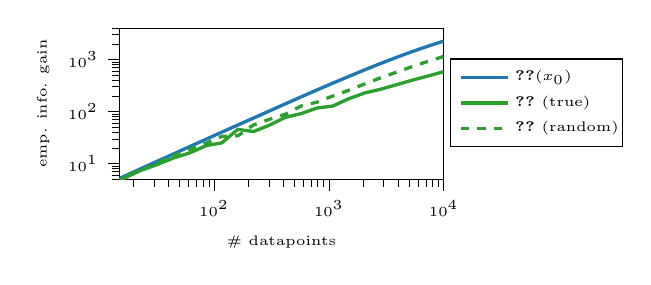
\begin{tikzpicture}

\definecolor{darkgray176}{RGB}{176,176,176}
\definecolor{darkorange25512714}{RGB}{255,127,14}
\definecolor{forestgreen4416044}{RGB}{44,160,44}
\definecolor{lightgray204}{RGB}{204,204,204}
\definecolor{steelblue31119180}{RGB}{31,119,180}



\begin{axis}[
width=5.7cm, height=3.5cm,
legend cell align={left},
legend style={
  at={(1.02,0.8)},
  anchor=north west,
},
tick align=outside,
tick pos=left,
x grid style={darkgray176},
xmin=15, xmax=10000,
xmode=log,
xlabel = {\text{\tiny \# datapoints}},
ylabel = {\text{\tiny emp. info. gain}},
xtick style={color=black},
xtick={0.01,0.1,1,10,100,1000,10000,100000,1000000},
xticklabels={
  \(\displaystyle {10^{-2}}\),
  \(\displaystyle {10^{-1}}\),
  \(\displaystyle {10^{0}}\),
  \(\displaystyle {10^{1}}\),
  \(\displaystyle {10^{2}}\),
  \(\displaystyle {10^{3}}\),
  \(\displaystyle {10^{4}}\),
  \(\displaystyle {10^{5}}\),
  \(\displaystyle {10^{6}}\)
},
y grid style={darkgray176},
ymin=5, ymax=4000,
ymode=log,
ytick style={color=black},
ytick={0.01,0.1,1,10,100,1000,10000,100000},
yticklabels={
  \(\displaystyle {10^{-2}}\),
  \(\displaystyle {10^{-1}}\),
  \(\displaystyle {10^{0}}\),
  \(\displaystyle {10^{1}}\),
  \(\displaystyle {10^{2}}\),
  \(\displaystyle {10^{3}}\),
  \(\displaystyle {10^{4}}\),
  \(\displaystyle {10^{5}}\)
},
yticklabel style = {font = \tiny},
xticklabel style = {font = \tiny},
]
\addplot [very thick, steelblue31119180,]
table {%
9999 2264.11377853996
7278 1804.26327966419
5298 1420.04472403012
3856 1095.40602083438
2807 836.680567640406
2043 631.775979654692
1487 472.562066757352
1082 352.135588183581
788 260.479692402163
573 191.711486161951
417 140.513623368777
303 102.644311381288
221 75.2133200772773
161 55.159666675983
117 40.2831954700074
85 29.31805807427
62 21.4780064745164
45 15.586340006635
32 11.0902089995822
23 7.97107383279624
17 5.89163232362588
12 4.15888308335967
9 3.11916231251975
6 2.07944154167984
4 1.38629436111989
3 1.03972077083992
2 0.693147180559945
1 0.346573590279973
1 0.346573590279973
1 0.346573590279973
};
\addlegendentry{\tiny \ref{eq:SDK}$(\bm{x}_0)$}
\addplot [very thick, forestgreen4416044, ]
table {%
9999 584.656726983284
7278 482.648758569247
5298 400.018580700851
3856 327.016416026596
2807 267.936837961897
2043 227.51171555213
1487 176.282258165846
1082 127.923214142905
788 116.989659625437
573 91.4829039943821
417 77.3576902555283
303 54.7094047705121
221 41.356397075653
161 45.5260312182046
117 25.0994743235434
85 22.1324167310142
62 16.1900860183269
45 12.9863449371233
32 9.59705643999886
23 7.41139449351921
17 5.41375041363105
12 3.95743297067132
9 3.10929738877
6 2.03296155184543
4 1.38344518620096
3 0.987590703724384
2 0.687289146233464
1 0.346573590279973
1 0.346573590279973
1 0.346573590279973
};
\addlegendentry{\tiny \textbf{\ref{eq:KE-SDK}} (true)}

\addplot [very thick, forestgreen4416044, dashed]
table {%
9999 1150.24144167382
7278 921.876964566388
5298 730.129320722141
3856 569.321298285514
2807 444.464772609148
2043 338.563956158658
1487 256.820764550324
1082 199.371251263352
788 151.518582913528
573 128.056611743859
417 88.4672878074439
303 70.909756169937
221 55.4035601061034
161 34.2302972124705
117 33.418917895361
85 24.5881170687663
62 18.9084220075427
45 14.4666214371714
32 10.138627472861
23 7.38739589901983
17 5.79102868865375
12 4.13377361608335
9 3.02188727225571
6 1.93259562627923
4 1.38548323020342
3 1.00804375391702
2 0.69309479616628
1 0.346573590279973
1 0.346573590279973
1 0.346573590279973
};
\addlegendentry{\tiny \textbf{\ref{eq:KE-SDK}} (random)$\!\!\!$}

\end{axis}

\end{tikzpicture}

    \vspace{-1.5\intextsep}
    \caption{Empirical information gain $\hat{\gamma}$ for a 2D linear system scaled to remove effects of constants. %
    The improved rates confirm our theoretical results for Koopman-equivariant GPs, leading to a lower information gain compared to their non-equivariant counterpart \eqref{eq:SDK}, even when a randomly sampled eigenvalue spectrum $\{\eig_j\}_{j=1}^D$  is used instead of the true spectrum.
    }
    \label{fig:enter-label}
\end{figure}
\textbf{Qualitative Comparison~~} We first qualitatively compare the different approaches on the predator-pray model as illustrated in Figure~\ref{fig:illustrative}. It can be clearly seen that all methods allow to accurately predict the future trajectory when given noise-free data from the dynamical system. However, when the state trajectories are perturbed by noise as commonly encountered in practice, significant differences between the predictions become apparent. While our proposed KE-GP maintains a high accuracy and reasonably small confidence intervals, the estimated uncertainty of the C-GP considerably grows and the prediction accuracy for longer horizons significantly drops for the Koopman operator regression (KOR) approach from \cite{Kostic2022LearningSpaces}. This high accuracy of KE-GPs can be attributed to their strong generalization capabilities captured by the information gain as discussed in Section \ref{section:analysisofsamplecomplexity}. When empirically comparing this value, we can immediately see an improvement over non-equivariant kernels, cf. Figure \ref{fig:enter-label}.\looseness=-1

\textbf{Quantitative Evaluation~~} We perform two evaluations for each model run and dataset: a small subset for which exact inference is possible and a large subset handled using variational inference. 
We observe that KE-GP performs robustly on all datasets and sizes as depicted in Tables~\ref{tab:smallsim} and \ref{tab:largesim}. While it consistently outperforms the C-GP, the KOR baseline is better on some datasets but the difference in accuracy is marginal. Importantly, KE-GPs provide a significant improvement over KOR for the other data sets. This is fully in line with our qualitative comparison, which shows that KOR can be sensitive to noise with a severe impact on its performance. In addition, we want to stress here that the KOR method does not come with methods for automated model selection, such that manual parameter tuning was necessary to make it competitive. Therefore, this comparison clearly demonstrates the improved generalization ability achieved by embedding the operator-theoretic foundations in our KE-GP approach.\looseness=-1

    
\section{CONCLUSION}
\label{sec:Concl}
We presented a novel approach to incorporate an operator-theoretic dynamical system structure into Gaussian process regression. Our framework enables a tractable probabilistic treatment of continuous-time dynamical models not present in existing literature. Utilizing a symmetrization tailored to dynamical systems, based on the concept of Koopman-equivariance (KE), we achieve a sample-complexity reduction compared to a contextual kernel without our proposed \eqref{eq:KoopObs} structure. In scaling to large datasets we exploit our model structure to avoid sampling any time/context-related inducing points. Hence, it does not suffer from a lack of correlation between inducing points, which is common for conventional sparse GP.
Through numerical experiments, we show the utility of our KE-GP, demonstrating superior prediction performance to vanilla contextual GPs and on par or better than Koopman operator learning. 


\subsubsection*{Acknowledgements}
This work is supported by the DAAD programme Konrad Zuse Schools of Excellence in Artificial Intelligence (relAI), sponsored by the German Federal Ministry of Education and Research and by the European Research Council (ERC) Consolidator Grant “Safe data-driven control for human-centric systems (CO-MAN)” under grant agreement number 864686.















% \documentclass[twoside]{article}

% \usepackage{aistats2025}
% If your paper is accepted, change the options for the package
% aistats2025 as follows:
%
%\usepackage[accepted]{aistats2025}
%
% This option will print headings for the title of your paper and
% headings for the authors names, plus a copyright note at the end of
% the first column of the first page.

% If you set papersize explicitly, activate the following three lines:
%\special{papersize = 8.5in, 11in}
%\setlength{\pdfpageheight}{11in}
%\setlength{\pdfpagewidth}{8.5in}

% If you use natbib package, activate the following three lines:
%\usepackage[round]{natbib}
%\renewcommand{\bibname}{References}
%\renewcommand{\bibsection}{\subsubsection*{\bibname}}

% If you use BibTeX in apalike style, activate the following line:
%\bibliographystyle{apalike}

% \begin{document}

% If your paper is accepted and the title of your paper is very long,
% the style will print as headings an error message. Use the following
% command to supply a shorter title of your paper so that it can be
% used as headings.
%
%\runningtitle{I use this title instead because the last one was very long}

% If your paper is accepted and the number of authors is large, the
% style will print as headings an error message. Use the following
% command to supply a shorter version of the authors names so that
% they can be used as headings (for example, use only the surnames)
%
%\runningauthor{Surname 1, Surname 2, Surname 3, ...., Surname n}

% Supplementary material: To improve readability, you must use a single-column format for the supplementary material.
\onecolumn
\appendix
\aistatstitle{From Deep Additive Kernel Learning to Last-Layer \\ Bayesian Neural Networks via Induced Prior Approximation: \\
Supplementary Materials}

\section{SPARSE CHOLESKY DECOMPOSITION}
\label{sec:sparse chol decompose}
In this section, we present the algorithm for constructing the induced grids $\mathbf{U}$ as defined in \cref{eq:GPlayer} by using sorted dyadic points, and obtaining the sparse Choleksy decomposition of the Laplace kernel in one dimension, as proposed in \citep{ding2024sparse}.

A set of one-dimensional level-$L$ dyadic points $\Xv_L$ in increasing order over the interval $[0,1]$ is defined as:
\begin{align}
    \Xv_{L}:= \left\{ \frac{1}{2^{L}}, \frac{2}{2^{L}}, \frac{3}{2^{L}}, \ldots, \frac{2^{L}-1}{2^{L}} \right\}.
\end{align}
However, this increasing order does not yield a sparse representation of the Markov kernel $k(\cdot,\cdot)$ on the points $\Xv_L$, i.e., Cholesky decomposition of the covariance matrix $k(\Xv_L, \Xv_L)$ is not sparse. To achieve a sparse hierarchical expansion, we first sort the dyadic points $\Xv_L$ according to their levels.

\paragraph{Sorted Dyadic Points}
For level-$\ell$ dyadic points $\Xv_{\ell}$ where $ \ell=1,\ldots,L$, we first define the set $\rho(\ell)$ consisting of odd numbers as follows:
\begin{align}
    \rho(\ell) = \left\{ 1,3,5,\ldots,2^{\ell}-1 \right\}.
\end{align}
Next, we define the sorted incremental set $\Dv_{\ell}$ (with $\Xv_{0}:= \varnothing$) as:
\begin{align}
    \Dv_{\ell} = 
    \left\{ \frac{i}{2^{\ell}}: i\in \rho(\ell) \right\} = \Xv_{\ell} - \Xv_{\ell-1}, \quad  \ell=1,\ldots L.
\end{align}
Thus, the level-$L$ dyadic points $\Xv_L$ can be decomposed into disjoint incremental sets $\{ \Dv_{\ell} \}_{\ell=1}^{L}$:
\begin{align}
    \Xv_{L} = \cup_{\ell=1}^{L} \Dv_{\ell}, \quad \Dv_{i} \cap \Dv_{j} = \varnothing \text{ for $i\neq j$}.
\end{align}
Therefore, we can define the sorted level-$L$ dyadic points using these incremental sets as:
\begin{align}\label{eq:sorted dyadic}
    \Xv_{L}^{\text{sort}}:= \left\{ \Dv_1,\Dv_2, \ldots, \Dv_{L} \right\} 
    = \left\{ \frac{i \in \rho(\ell) }{2^{\ell}}, \ell=1,\ldots,L \right\}.
\end{align}
For example, the sorted level-3 dyadic points are given by:
\begin{align}
    \Xv_{3}^{\text{sort}} 
    = \bigg\{ 
    \begingroup
        \color{blue}
        \underbracket{
            \color{black}
            \frac{1}{2^1}
        }_{\color{blue}
            \Dv_1
        }
    \endgroup
    , 
    \begingroup
        \color{blue}
        \underbracket{
            \color{black}
            \frac{1}{2^2}, \frac{3}{2^2}
        }_{\color{blue}
            \Dv_2
        }
    \endgroup
    ,
    \begingroup
        \color{blue}
        \underbracket{
            \color{black}
            \frac{1}{2^3}, \frac{3}{2^3}, \frac{5}{2^3}, \frac{7}{2^3}
        }_{\color{blue}
            \Dv_3
        }
    \endgroup
     \bigg\}.
\end{align}

\paragraph{Algorithm}
We now present the algorithm for computing the inverse of the upper triangular Cholesky factor $[ \Lv_{\Xv_{L}^{\text{sort}}}^{\top} ]^{-1}$ of the covariance matrix $k(\Xv_{L}^{\text{sort}}, \Xv_{L}^{\text{sort}})$ in \Cref{alg:cholesky}, where $\Lv_{\Xv_{L}^{\text{sort}}} \Lv_{\Xv_{L}^{\text{sort}}}^{\top} = k(\Xv_{L}^{\text{sort}}, \Xv_{L}^{\text{sort}})$.. The corresponding proof can be found in \citep{ding2024sparse}. The output of \Cref{alg:cholesky} is a sparse matrix with $\Oc(3 \cdot (2^{L}-1))$ nonzero entries. Since each iteration of the for-loop only requires solving a $3 \times 3$ linear system, which costs $\Oc(3^3)$ time, the total computational complexity of \Cref{alg:cholesky} is $\Oc(2^L-1)$. This implies that the complexity of computing $\left[ \Lv_{\Uv}^{\top} \right]^{-1}$ in \cref{eq:GPlayer} is $\Oc(M)$ when $\Uv$, the induced grid of size $M$, consists of sorted dyadic points as defined in \cref{eq:sorted dyadic}.

\begin{algorithm}[hbt!]
\caption{Computation of the inverse Cholesky factor for the Markov kernel $k(\cdot, \cdot)$ on sorted one-dimensional level-$L$ dyadic points $\Xv_L^{\text{sort}}$.}
\label{alg:cholesky}
\setstretch{0.99} % set the line spacing to 0.99
\begin{algorithmic}[1]
    \STATE {\bfseries Input:} Markov kernel $k(\cdot,\cdot)$, sorted level-$L$ dyadic points $\Xv_{L}^{\text{sort}}$
    \STATE {\bfseries Output:} inverse of the upper triangular Cholesky factor $\Rv:= [ \Lv_{\Xv_{L}^{\text{sort}}}^{\top} ]^{-1}$, s.t. $\Lv_{\Xv_{L}^{\text{sort}}} \Lv_{\Xv_{L}^{\text{sort}}}^{\top} = k(\Xv_{L}^{\text{sort}}, \Xv_{L}^{\text{sort}})$
    \STATE Initialize $\Rv \leftarrow \text{zeros($2^L-1$,$2^L-1$)}$;
    \STATE Define $k(\pm \infty, \cdot) = k(\cdot, \pm \infty) = 0$;
    \FOR{$\ell=1$ {\bfseries to} $L$}
        \FOR{$i \in \rho(\ell)=\{1,3,\ldots,2^{\ell}-1\}$}
            \STATE $x_{\text{mid}} := \frac{i}{2^{\ell}}$;\quad
            $x_{\text{left}}:=\frac{i-1}{2^{\ell}}$ {\bfseries if} $i>1$ {\bfseries else} $-\infty$;\quad
            $x_{\text{right}}:=\frac{i+1}{2^{\ell}}$ {\bfseries if} $i<2^{\ell}-1$ {\bfseries else} $+\infty$;
            \STATE Get $i_{\text{mid}}$, $i_{\text{left}}$, $i_{\text{right}}$, the indices of the points $x_{\text{mid}}$, $x_{\text{left}}$, $x_{\text{right}}$ in the sorted set $\Xv_{L}^{\text{sort}}$ respectively;
            \STATE Get the coefficients $c_1$, $c_2$, $c_3$ by solving the following linear system:
            \begin{align}
                \begin{bmatrix}
                     & k(x_{\text{left}}, x_{\text{left}})
                     & k(x_{\text{left}}, x_{\text{mid}})
                     & k(x_{\text{left}}, x_{\text{right}}) \\
                     & k(x_{\text{mid}}, x_{\text{left}})
                     & k(x_{\text{mid}}, x_{\text{mid}})
                     & k(x_{\text{mid}}, x_{\text{right}}) \\
                     & k(x_{\text{right}}, x_{\text{left}})
                     & k(x_{\text{right}}, x_{\text{mid}})
                    &k(x_{\text{right}}, x_{\text{right}})
                \end{bmatrix}
                \begin{bmatrix}
                    c1\\
                    c2\\
                    c3
                \end{bmatrix}=
                \begin{bmatrix}
                    0\\
                    1\\
                    0
                \end{bmatrix}.
            \end{align}
            \STATE $[c_1,c_2,c_3] := [c_1,c_2,c_3] / \sqrt{c_2}$;
            \STATE {\bfseries if} $x_{\text{left}} \neq - \infty$, 
            {\bfseries then} $\Rv[i_{\text{left}} ,i_{\text{mid}}] = c_1$; \quad
            {\bfseries if} $x_{\text{right}} \neq + \infty$, 
            {\bfseries then} $\Rv[i_{\text{right}} ,i_{\text{mid}}] = c_3$;
            \STATE $\Rv[i_{\text{mid}} ,i_{\text{mid}}] = c_2$;
        \ENDFOR
    \ENDFOR
\end{algorithmic}
\end{algorithm}


\section{REPARAMETERIZATION OF KERNEL LENGTHSCALES}
\label{sec:theo}
Considering the additive Laplace kernel with fixed lengthscale $\tilde{\theta}$ for all base kernels, applying linear projections $\left\{ \wv_{p}^{\top}\xv \right\}_{p=1}^{P}$ on inputs $\xv\in \Rb^D$ will give:
\begin{align}
    &\sum_{p=1}^{P}\sigma^2_p k_p\left( \wv^{\top}_{p}\xv,\wv^{\top}_{p}\xv^{\prime} \right)\nonumber \\
    = & \sum_{p=1}^{P} \sigma^2_p\exp \left( -  \frac{\sum_{d=1}^{D} \left| w_{p,d}\left( x_{d}-x_{d}^{\prime} \right) \right|}{\tilde{\theta}} \right)\nonumber \\
    = & \sum_{p=1}^{P} \prod_{d=1}^{D} \sigma^2_p\exp \left( - \frac{\left| x_{d}-x_{d}^{\prime} \right|}{\tilde{\theta} / \left| w_{p,d}\right| } \right)\nonumber \\
    = & \sum_{p=1}^{P} \prod_{d=1}^{D} \sigma^2_p\exp \left( - \frac{\left| x_{d}-x_{d}^{\prime} \right|}{\theta_{p,d}} \right),
\end{align}
This still leads to an additive Laplace kernel but with adaptive lengthscale $\theta_{p,d}$ for base kernels. The resulting kernel also retains \emph{sparse} Cholesky decomposition by the properties of Markov kernels so that the complexity of inference is $\Oc(M)$.

\section{INFERENCE OF PREDICTIVE DISTRIBUTION}
\label{sec:uq of inference}
Given an input $\xv \in \Rb^D$, the prediction of the DAK model can be written in the following equation according to \cref{eq:DAK prediction}: 
\begin{align}
    \tilde{f}_{\xv}
    &= \sum_{p=1}^{P}
    \sigma_p \Big(
        \phi(h_{\psi}^{[p]}(\xv)) \zv_p
    \Big) + \mu \nonumber\\
    &= \sum_{p=1}^{P}
    \sigma_p \Big(
        \bm{\phi}_{p}^{\top} \zv_p
    \Big) + \mu,
\end{align}
where $\bm{\phi}_{p}^{\top}:=\phi(h_{\psi}^{[p]}(\xv)) \in \Rb^{1 \times M}$
% , $\mu_p:=\mu_p(h_{\psi}^{[p]}(\xv)) \in \Rb$
. We assume the variational distribution over the independent Gaussian weights $\zv_p \sim \Nc(\bm{m}_{\zv_p}, \Sv_{\zv_p})$ and the bias $\mu \sim \Nc(m_{\mu}, \sigma_{\mu}^2)$. Then it's straighforward to deduce that
\begin{align}
    \bm{\phi}_{p}^{\top} \zv_p + \mu 
    &\sim
    \Nc\left(
    \bm{\phi}_{p}^{\top} \bm{m}_{\zv_p} + m_{\mu},\hspace{0.2em}
    \bm{\phi}_{p}^{\top} \Sv_{\zv_p} \bm{\phi}_{p} + \sigma_{\mu}^2
    \right), \\
    \sigma_p \left(
    \bm{\phi}_{p}^{\top} \zv_p 
    \right) + \mu
    & \sim
    \Nc\left(
    \sigma_p ( \bm{\phi}_{p}^{\top} \bm{m}_{\zv_p} )+ m_{\mu} ,\hspace{0.2em}
    \sigma_p^2( \bm{\phi}_{p}^{\top} \Sv_{\zv_p} \bm{\phi}_{p}) + \sigma_{\mu}^2
    \right), \\
    \tilde{f}_{\xv} = 
    \sum_{p=1}^{P}
    \sigma_p \left(
    \bm{\phi}_{p}^{\top} \zv_p
    \right) + \mu
    & \sim
    \Nc\left(
    \sum_{p=1}^{P}
    \sigma_p ( \bm{\phi}_{p}^{\top} \bm{m}_{\zv_p}) + m_{\mu} ,\hspace{0.2em}
    \sum_{p=1}^{P}
    \sigma_p^2( \bm{\phi}_{p}^{\top} \Sv_{\zv_p} \bm{\phi}_{p} ) + \sigma_{\mu}^2
    \right).
\end{align}
Therefore, we obtain the predictive distribution of the $\tilde{f}(\xv)$ at the point $\xv \in \Rb^D$ and its mean and variance are given by:
\begin{subequations}
\label{eq:dak inference closed form}
\begin{align}
    \Eb\left[ \tilde{f}_{\xv} \right]
        = \sum_{p=1}^{P}
        \sigma_p ( \bm{\phi}_{p}^{\top} \bm{m}_{\zv_p}) + m_{\mu},
\end{align}
\begin{align}
    \text{Var}\left[ \tilde{f}_{\xv} \right]
        =\sum_{p=1}^{P}
        \sigma_p^2( \bm{\phi}_{p}^{\top} \Sv_{\zv_p} \bm{\phi}_{p}) + \sigma_{\mu}^2.
\end{align}
\end{subequations}
% \begin{subequations}
% \label{eq:dak inference closed form}
%     \begin{align}
%         \Eb\left[ \tilde{f}(\xv) \right]
%         = \sum_{p=1}^{P}
%         \sigma_p ( \bm{\phi}_{p}^{\top} \bm{m}_{\zv_p} + m_{\mu_p} ),
%     \end{align}
%     \begin{align}
%         \text{Var}\left[ \tilde{f}(\xv) \right]
%         =\sum_{p=1}^{P}
%         \sigma_p^2( \bm{\phi}_{p}^{\top} \Sigma_{\zv_p} \bm{\phi}_{p} + \sigma_{\mu_p}^2).
%     \end{align}
% \end{subequations}


\section{TRAINING OF VARIATIONAL INFERENCE}
\label{sec:training}
Given the dataset $\mathcal{D}=\{ \Xv, \yv \}$ where $\Xv:=\{ \xv_i \}_{i=1}^N$, $\yv=(y_1,\ldots,y_N)^{\top}$, $\xv_i \in \Rb^D$, $y_i\in\Rb$, the prediction $\tilde{f}_{\Xv}\in \Rb^N$ of DAK is given by all the parameters $\bm{\theta}=\left\{ \psi, \bm{\sigma} \right\}$, $\bm{\eta}=\left\{ \{ \mv_{\zv_{p}},\Sv_{\zv_{p}}\}_{p=1}^{P} , \{m_{\mu},\sigma_{\mu} \} \right\}$ according to \cref{eq:DAK prediction}:
\begin{align}
    \tilde{f}_{\Xv}:= \tilde{f}(\Xv; \bm{\theta}, \bm{\eta})
    = \sum_{p=1}^{P}
    \sigma_p \Big(
        \phi(h_{\psi}^{[p]}(\Xv)) \zv_p
    \Big) + \mu,
\end{align}
where $\zv_{p} \sim \mathcal{N} (\bm{m}_{\zv_p} ,\Sv_{\zv_p})$, $p=1,\ldots,P$, and $\mu \sim \mathcal{N} ( m_{\mu},\sigma^2_{\mu} )$ are variational variables $\Theta_{\text{var}}$ parameterized by $\bm{\eta}$. The variational distribution is denoted by $q_{\bm{\eta}}(\Theta_{\text{var}})= q(\mu)\prod_{p=1}^{P} q(\zv_{p}) = \Nc ( m_{\mu} ,\sigma_{\mu}^2 )\prod_{p=1}^{P} 
\Nc ( \bm{m}_{\zv_p} ,\Sv_{\zv_p} )$, and the variational prior is denoted by $p(\Theta_{\text{var}})$.

We consider the KL divergence between $q_{\bm{\eta}}(\Theta_{\text{var}})$ and the true posterior $p(\Theta_{\text{var}}\vert \yv, \Xv, \bm{\theta})$:
\begin{align}
& \qquad \text{KL} \left[ q_{\bm{\eta}}(\Theta_{\text{var}}) \| p(\Theta_{\text{var}} \vert \yv,\Xv, \bm{\theta} ) \right] \nonumber \\
= & \int q_{\bm{\eta}}(\Theta_{\text{var}} )\log \frac{q_{\bm{\eta}}(\Theta_{\text{var}} )}{p(\Theta_{\text{var}} \vert \yv,\Xv,\bm{\theta} )} d\Theta_{\text{var}} \nonumber \\
= & \int q_{\bm{\eta}}(\Theta_{\text{var}} )\log \frac{q_{\bm{\eta}}(\Theta_{\text{var}} )p(\yv \vert \Xv,\bm{\theta})}{p(\yv \vert \Xv,\bm{\theta} ,\Theta_{\text{var}} )p(\Theta_{\text{var}} )} d\Theta_{\text{var}} \nonumber \\
= & \int q_{\bm{\eta}}(\Theta_{\text{var}} )\log \frac{q_{\bm{\eta}}(\Theta_{\text{var}} )}{p(\Theta_{\text{var}} )} d\Theta_{\text{var}} -\int q_{\bm{\eta}}(\Theta_{\text{var}} )\log p(\yv \vert \tilde{f}_{\Xv} )d\Theta_{\text{var}} +\log p(\yv\vert \Xv,\bm{\theta}).
\end{align}
Using the fact that $\text{KL}[\cdot \| \cdot] \geq 0$, we have
\begin{align}
\label{eq:variational lower bound}
    \log p(\yv\vert \Xv,\bm{\theta}) & \geq \int q_{\bm{\eta}}(\Theta_{\text{var}} )\log p(\yv \vert \tilde{f}_{\Xv} )d\Theta_{\text{var}} - \text{KL} \left[ q_{\bm{\eta}}(\Theta_{\text{var}} ) \| p(\Theta_{\text{var}}) \right] \nonumber \\
    & = \Eb_{q_{\bm{\eta}}(\Theta_{\text{var}} )} \left[ \log p(\yv \vert \tilde{f}_{\Xv} ) \right] - \text{KL} \left[ q_{\bm{\eta}}(\Theta_{\text{var}} ) \| p(\Theta_{\text{var}}) \right].
\end{align}

\paragraph{Full-training.}
Firstly, we present the joint training of $\bm{\theta}$ and $\bm{\eta}$. The most common approach optimizes the marginal log-likelihood (the left-hand side of \cref{eq:variational lower bound}):
\begin{align}
    \bm{\theta}^{\ast} &=\argmax_{\bm{\theta}} \log p(\yv\vert \Xv,\bm{\theta} ) \\
    &= \argmax_{\bm{\theta}} \log \int p\left( y\vert X,\bm{\theta},\Theta_{\text{var}} \right) p(\Theta_{\text{var}})d\Theta_{\text{var}},
\end{align}
which involves intractable integral in some tasks such as classification. Instead, we optimize the variational lower bound (the right-hand side of \cref{eq:variational lower bound}):
\begin{align}
    \Theta^{\ast} := \argmax_{\bm{\theta},\bm{\eta}} \mathcal{L}(\bm{\theta},\bm{\eta}) =\argmax_{\bm{\theta},\bm{\eta}}\left\{ E_{q_{\bm{\eta}}(\Theta_{\text{var}} )}\left[ \log p(\yv|\tilde{f}_{\Xv} ) \right] -\text{KL} \left[ q_{\bm{\eta}}(\Theta_{\text{var}} )\| p(\Theta_{\text{var}} ) \right] \right\}.
\end{align}

\paragraph{Fine-tuning.}
An alternative training approach is to firstly pre-train the deterministic parameters of feature extractor by standard neural network training, with mean squared error for regression or cross-entropy for classification as the loss function, and then fine-tune the last layer additive GP with fixed features. The objective function is identical to \cref{eq:elbo}, but $\bm{\theta}$ is learned during the pre-training step and is no longer optimized during fine-tuning.


\section{ELBO}%{DERIVATION OF ELBO}
\label{sec:elbo}
\subsection{Assumptions}
Consider the model $y_i = \tilde{f}(\xv_i) + \epsilon_i$ with the i.i.d. noise $\epsilon_i \overset{\text{i.i.d.}}{\sim} \Nc(0, \sigma_{f}^2)$ and $\tilde{f} : \Rb^D \rightarrow \Rb$ is defined in \cref{eq:DAK prediction}. The training dataset is $\mathcal{D} = \{ \Xv, \yv \}$ where $\Xv:=\{ \xv_i \}_{i=1}^N$, $\yv=(y_1,\ldots,y_N)^{\top}$, $\xv_i \in \Rb^D$, $y_i\in\Rb$. $\Theta_{\text{var}}:= \{ \mu ,\{ \zv_{p}\}_{p=1}^{P} \}$ are the variational random variables consisting of Gaussian weights and bias of $P$ units, $\psi$ are the parameters of the NN, $\bm{\sigma}:=(\sigma_1, \ldots, \sigma_p)^{\top}$ are the scale parameters of base GP layers. The variational distributions are $q(\mu)=\Nc(m_{\mu}, \sigma_{\mu}^2)$, $q(\zv_p)=\Nc(\bm{m}_{\zv_p}, \Sv_{\zv_p})$ and the variational priors are $p(\mu)=\Nc(\check{m}_{\mu} ,\check{\sigma}^2_{\mu})$, $p(\zv_p)=\Nc(\check{\bm{m}}_{\zv_p} ,\check{\Sv}_{\zv_p})$. Note that $\Sv_{\zv_p}\in\Rb^{M \times M}$ is a diagonal covariance matrix due to the independence of $\zv_p$, $M$ is the number of inducing points $\Uv$ defined in \cref{eq:GPlayer}, and $\bm{m}_{\zv_p} \in \Rb^M$, $m_{\mu} \in \Rb$, $\sigma_{\mu}^2 \in \Rb$. We derive the ELBO in VI to learn the preditive posterior over the variational variables $\Theta_{\text{var}}:= \{ \mu ,\{ \zv_{p}\}_{p=1}^{P} \}$ parameterized by $\bm{\eta}:=\left\{ \{ \mv_{\zv_{p}},\Sv_{\zv_{p}}\}_{p=1}^{P} , \{m_{\mu},\sigma_{\mu} \} \right\}$, and optimize the deterministic parameters $\bm{\theta}:=\{\psi, \bm{\sigma}\}$.

\subsection{Expected Log Likelihood}
\paragraph{Closed Form}
The \emph{expected log likelihood}, which is the first term in ELBO defined in \cref{eq:elbo}, is given by 
\begin{align}
    {\Eb}_{q_{\bm{\eta}}(\Theta_{\text{var}})} \left[ \log \text{Pr} (\yv \vert \tilde{f}_{\Xv} ) \right]
    &= {\Eb}_{q_{\bm{\eta}}(\Theta_{\text{var}})} \left[ 
    \log \prod_{i=1}^{N} 
    p (y_i \vert \tilde{f}_{\xv_i} )
    \right] \nonumber\\
    &= \sum_{i=1}^{N} 
    {\Eb}_{q_{\bm{\eta}}(\Theta_{\text{var}})} \left[ 
    \log
    p (y_i \vert \tilde{f}_{\xv_i} )
    \right] \nonumber\\
    &= \sum_{i=1}^{N} 
    {\Eb}_{q_{\bm{\eta}}(\Theta_{\text{var}})} \left[ 
    \log
    \Nc( \tilde{f}_i,\hspace{0.2em} \sigma_{f}^2 )
    \right] \nonumber\\
    &= \sum_{i=1}^{N} 
    {\Eb}_{q_{\bm{\eta}}(\Theta_{\text{var}})} \left[ 
    \log \left(
    (2\pi \sigma_{f}^2)^{-\frac{1}{2}}
    \exp\left\{  
        -\frac{ (y_i - \tilde{f}_i)^2 }{2 \sigma_{f}^2}
    \right\}
    \right)
    \right] \nonumber\\
    &= \sum_{i=1}^{N} 
    {\Eb}_{q_{\bm{\eta}}(\Theta_{\text{var}})} \left[
    -\frac{1}{2} \log(2\pi) 
    - \frac{1}{2}\log(\sigma_{f}^2)
    - \frac{1}{2 \sigma_{f}^2}
    (y_i - \tilde{f}_i)^2
    \right] \nonumber\\
    &= - \frac{N}{2} \log(2\pi)
    - \frac{N}{2} \log(\sigma_{f}^2)
    - \frac{1}{2 \sigma_{f}^2}
    \sum_{i=1}^{N}
    {\Eb}_{q_{\bm{\eta}}(\Theta_{\text{var}})} \left[
    (y_i - \tilde{f}_i)^2
    \right] \nonumber\\
    &= - \frac{N}{2} \log(2\pi)
    - \frac{N}{2} \log(\sigma_{f}^2)
    - \frac{1}{2 \sigma_{f}^2}
    \sum_{i=1}^{N} \left(
    \left({\Eb}_{q(\Theta_{\text{var}})} \left[
    (y_i - \tilde{f}_i)
    \right] \right)^2
    + \text{Var}_{q(\Theta_{\text{var}})} \left[
    (y_i - \tilde{f}_i)
    \right]
    \right) \label{eq:evidence halfway},
\end{align}
where
\begin{align}
    \tilde{f}_i
    % \mu_{\tilde{f}_i} &:= \tilde{f}(\xv_i;\Theta_{\text{var}}, \Theta_{\text{det}} ) \nonumber\\
    &= \sum_{p=1}^{P} \sigma_p \Big(
    \begingroup
        \color{blue}
        \underbracket{
            \color{black}
            \phi(h_{\psi}^{[p]}(\xv_i))
        }_{\color{blue}
            :=\bm{\phi}_{i,p}^{\top} \in \Rb^{1 \times M}
        }
    \endgroup
    \zv_p
    \Big)
    + \mu
    % \begingroup
    %     \color{blue}
    %     \underbracket{
    %         \color{black}
    %         \mu_{p}(h_{\psi}^{[p]}(\xv_i))
    %     }_{\color{blue}
    %         :=\mu_{i,p} \in \Rb
    %     }
    % \endgroup 
    \nonumber\\
    &= \sum_{p=1}^{P} \sigma_p \left(
    \bm{\phi}_{i,p}^{\top} \zv_p 
    \right) + \mu.
\end{align}
Recall that the variational assumptions $q(\zv_p)=\Nc(\bm{m}_{\zv_p}, \Sv_{\zv_p})$ and $q(\mu)=\Nc(m_{\mu}, \sigma_{\mu}^2)$, we can infer that
\begin{align}
    \bm{\phi}_{i,p}^{\top} \zv_p + \mu 
    &\sim
    \Nc\left(
    \bm{\phi}_{i,p}^{\top} \bm{m}_{\zv_p} + m_{\mu},\hspace{0.2em}
    \bm{\phi}_{i,p}^{\top} \Sv_{\zv_p} \bm{\phi}_{i,p} + \sigma_{\mu}^2
    \right), \\
    \sigma_p \left(
    \bm{\phi}_{i,p}^{\top} \zv_p 
    \right) + \mu
    & \sim
    \Nc\left(
    \sigma_p ( \bm{\phi}_{i,p}^{\top} \bm{m}_{\zv_p} ) + m_{\mu},\hspace{0.2em}
    \sigma_p^2( \bm{\phi}_{i,p}^{\top} \Sv_{\zv_p} \bm{\phi}_{i,p} ) + \sigma_{\mu}^2
    \right), \\
    \tilde{f}_i = 
    \sum_{p=1}^{P}
    \sigma_p \left(
    \bm{\phi}_{i,p}^{\top} \zv_p 
    \right)+ \mu
    & \sim
    \Nc\left(
    \sum_{p=1}^{P}
    \sigma_p ( \bm{\phi}_{i,p}^{\top} \bm{m}_{\zv_p} )+ m_{\mu},\hspace{0.2em}
    \sum_{p=1}^{P}
    \sigma_p^2( \bm{\phi}_{i,p}^{\top} \Sv_{\zv_p} \bm{\phi}_{i,p} ) + \sigma_{\mu}^2
    \right), \\
    y_i - \tilde{f}_i
    & \sim 
    \Nc\left(
    y_i - 
    \sum_{p=1}^{P}
    \sigma_p ( \bm{\phi}_{i,p}^{\top} \bm{m}_{\zv_p} ) -m_{\mu},\hspace{0.2em}
    \sum_{p=1}^{P}
    \sigma_p^2( \bm{\phi}_{i,p}^{\top} \Sv_{\zv_p} \bm{\phi}_{i,p} ) + \sigma_{\mu}^2
    \right).
\end{align}
Therefore, 
\begin{subequations}\label{eq:exp and var in evidence}
    \begin{align}
        \left({\Eb}_{q(\Theta_{\text{var}})} \left[
        (y_i - \tilde{f}_i)
        \right] \right)^2
        = \left(
         y_i - 
        \sum_{p=1}^{P}
        \sigma_p ( \bm{\phi}_{i,p}^{\top} \bm{m}_{\zv_p} ) -m_{\mu}
        \right)^2,
    \end{align}
    \begin{align}
        \text{Var}_{q(\Theta_{\text{var}})}
        \left[
        (y_i - \tilde{f}_i)
        \right]
        = \sum_{p=1}^{P}
        \sigma_p^2( \bm{\phi}_{i,p}^{\top} \Sv_{\zv_p} \bm{\phi}_{i,p} ) + \sigma_{\mu}^2.
    \end{align}
\end{subequations}
By applying \cref{eq:exp and var in evidence} to \cref{eq:evidence halfway}, we derive the analytical formula for the expected evidence, expressed as
\begin{align}
    {\Eb}_{q_{\bm{\eta}}(\Theta_{\text{var}})} \left[ \log \text{Pr} (\yv \vert \tilde{f}_{\Xv} ) \right]
    &= - \frac{N}{2} \log(2\pi)
    - \frac{N}{2} \log(\sigma_{f}^2) \nonumber\\
    &- \frac{1}{2 \sigma_{f}^2}
    \sum_{i=1}^{N} \left(
        \Big(
         y_i - 
        \sum_{p=1}^{P}
        \sigma_p ( \bm{\phi}_{i,p}^{\top} \bm{m}_{\zv_p} ) -m_{\mu}
        \Big)^2
        + \sum_{p=1}^{P}
        \sigma_p^2( \bm{\phi}_{i,p}^{\top} \Sv_{\zv_p} \bm{\phi}_{i,p} )+ \sigma_{\mu}^2
    \right). \label{eq:evidence final}
\end{align}

\paragraph{Monte Carlo Approximation}
For comparison, we provide the equation for computing the Monte Carlo estimate of the ELBO in the paragraph that follows.
\begin{align}
    {\Eb}_{q_{\bm{\eta}}(\Theta_{\text{var}})} \left[ \log \text{Pr} (\yv \vert \tilde{f}_{\Xv} ) \right]
    % &= {\Eb}_{q(\Theta)} \left[ 
    % \log \prod_{i=1}^{N} 
    % p (y_i \vert \xv_i,\Theta, \psi, \bm{\sigma})
    % \right] \nonumber\\
    &= \sum_{i=1}^{N} 
    {\Eb}_{q_{\bm{\eta}}(\Theta_{\text{var}} )} \left[ 
    \log
    p (y_i \vert \tilde{f}_{\xv_i} )
    \right] \nonumber\\
    & \approx \sum_{i=1}^{N}
    \frac{1}{S}
     \sum_{s=1}^{S}
    \log
    p (y_i \vert \xv_i,\tilde{\Theta}^{(s)}_{\text{var}}, \bm{\theta} ) \nonumber\\
    &= \frac{1}{S} \sum_{i=1}^{N} 
    \sum_{s=1}^{S} 
    \log
    \Nc(y_i \left\vert\right. \tilde{f}_{i}^{(s)},\hspace{0.2em} \sigma_{f}^2 )
    \nonumber\\
    &= \frac{1}{S} \sum_{i=1}^{N} 
    \sum_{s=1}^{S} 
    \log \left(
    (2\pi \sigma_{f}^2)^{-\frac{1}{2}}
    \exp\left\{  
        -\frac{ (y_i - \tilde{f}_{i}^{(s)})^2 }{2 \sigma_{f}^2}
    \right\}
    \right)
    \nonumber\\
    &= \frac{1}{S} \sum_{i=1}^{N} 
    \sum_{s=1}^{S} \left(
    -\frac{1}{2} \log(2\pi) 
    - \frac{1}{2}\log(\sigma_{f}^2)
    - \frac{1}{2 \sigma_{f}^2}
    (y_i - \tilde{f}_{i}^{(s)})^2
    \right) \nonumber\\
    &= - \frac{N}{2} \log(2\pi)
    - \frac{N}{2} \log(\sigma_{f}^2)
    - \frac{1}{2 \sigma_{f}^2}
    \sum_{i=1}^{N}
    \frac{1}{S} \sum_{s=1}^{S}
    (y_i - \tilde{f}_{i}^{(s)})^2, \label{eq:evidence halfway mc approx}
\end{align}
where $S$ is the number of Monte Carlo samples, $\{  \tilde{\mu}^{(s)} ,\{ \tilde{\zv}_{p}^{(s)} \}_{p=1}^{P} \} := \tilde{\Theta}^{(s)}_{\text{var}}$ are the $s$-th Monte Carlo samplings over the variational parameters $\Theta_{\text{var}}$ and $\tilde{\Theta}^{(s)}_{\text{var}} \sim q_{\bm{\eta}}(\Theta_{\text{var}})$, $\tilde{f}_{i}^{(s)}$ is given as follows:
\begin{align}
    \tilde{f}_{i}^{(s)} &:= \tilde{f}(\xv_i;\tilde{\Theta}^{(s)}_{\text{var}},\bm{\theta} ) \nonumber\\
    &= \sum_{p=1}^{P} \sigma_p \Big(
    \begingroup
        \color{blue}
        \underbracket{
            \color{black}
            \phi(h_{\psi}^{[p]}(\xv_i))
        }_{\color{blue}
            :=\bm{\phi}_{i,p}^{\top} \in \Rb^{1 \times M}
        }
    \endgroup
    \tilde{\zv}_p^{(s)} 
    \Big) + \tilde{\mu}^{(s)} \nonumber\\
    &= \sum_{p=1}^{P} \sigma_p \left(
    \bm{\phi}_{i,p}^{\top} \tilde{\zv}_p^{(s)} 
    \right)+ \tilde{\mu}^{(s)}. \label{eq:mc approx mean}
\end{align}
Therefore, we plug \cref{eq:mc approx mean} into \cref{eq:evidence halfway mc approx} and get the the Monte Carlo estimate of the ELBO written in the following formula:
\begin{align}
    {\Eb}_{q_{\bm{\eta}}(\Theta_{\text{var}})} \left[ \log \text{Pr} (\yv \vert \tilde{f}_{\Xv} ) \right]
    &\approx
    - \frac{N}{2} \log(2\pi)
    - \frac{N}{2} \log(\sigma_{f}^2)
    - \frac{1}{2 \sigma_{f}^2}
    \sum_{i=1}^{N}
    \frac{1}{S} \sum_{s=1}^{S}
    \Big(y_i - 
    \sum_{p=1}^{P} \sigma_p \left(
    \bm{\phi}_{i,p}^{\top} \tilde{\zv}_p^{(s)} 
    \Big)- \tilde{\mu}^{(s)}
    \right)^2, \label{eq:evidence final mc approx} \\
    \tilde{\zv}_p^{(s)} &\sim \Nc(\bm{m}_{\zv_p}, \Sv_{\zv_p}),\qquad
    \tilde{\mu}^{(s)} \sim \Nc(m_{\mu}, \sigma_{\mu}^2).
\end{align}


\subsection{KL Divergence}
Since we place Gaussian assumptions over the variational parameters $\Theta_{\text{var}}$,  the \emph{KL divergence}, which is the second term in ELBO defined in \cref{eq:elbo}, is then given by
\begin{align}
    \text{KL} \left[ q(\Theta_{\text{var}} ) \| p(\Theta_{\text{var}}) \right]
    &= \text{KL} \left[ q( \mu ,\{ \zv_{p}\}_{p=1}^{P} ) \Vert p( \mu ,\{ \zv_{p}\}_{p=1}^{P}) \right] \nonumber\\
    & =  
    \text{KL} \left[ q(\mu) \Vert p(\mu) \right] 
    + \sum_{p=1}^{P} 
    \text{KL} \left[ q(\zv_{p}) \Vert p(\zv_{p}) \right],
\end{align}

\begin{align}
     \text{KL} \left[ q(\mu) \Vert p(\mu) \right]
     = \frac{1}{2} \left(
     \frac{\sigma_{\mu}^2}{\check{\sigma}_{\mu}^2} 
     + \frac{(m_{\mu} - \check{m}_{\mu})^2}{\check{\sigma}_{\mu}^2} 
     -\log\left( \frac{\sigma_{\mu}^2}{\check{\sigma}_{\mu}^2} \right)
     -1
     \right),
\end{align}

\begin{align}
    \text{KL} \left[ q(\zv_{p}) \Vert p(\zv_{p}) \right]
    = \frac{1}{2} \sum_{i=1}^{M} \left(
     \frac{[\Sv_{\zv_p}]_{ii}}{[\check{\Sv}_{\zv_p}]_{ii}} 
     + \frac{([\bm{m}_{\zv_p}]_{i} - [\check{\bm{m}}_{\zv_p}]_i)^2}{[\check{\Sv}_{\zv_p}]_{ii}}
     -\log\left( 
     \frac{[\Sv_{\zv_p}]_{ii}}{[\check{\Sv}_{\zv_p}]_{ii}}  
     \right)
     -1
     \right),
\end{align}
where $[\Sv_{\zv_p}]_{ii}$ is the $(i,i)$-th element of the diagonal covariance matrix $\Sv_{\zv_p} \in \Rb^{M \times M}$, $[\bm{m}_{\zv_p}]_{i}$ is the $i$-th element of the mean vector $\bm{m}_{\zv_p} \in \Rb^M$, the approximated posteriors are $q(\mu)=\Nc(m_{\mu}, \sigma_{\mu}^2)$, $q(\zv_p)=\Nc(\bm{m}_{\zv_p}, \Sv_{\zv_p})$ and the priors are $p(\mu)=\Nc(\check{m}_{\mu} ,\check{\sigma}^2_{\mu})$, $p(\zv_p)=\Nc(\check{\bm{m}}_{\zv_p} ,\check{\Sv}_{\zv_p})$.

% \subsection{Performance Comparison}
% \label{sec:toy exp compare}
% We compare the perforamce of computing the ELBO in \cref{eq:elbo} by using closed form in \cref{eq:evidence final} and using Monte Carlo approximation in \cref{eq:evidence final mc approx} in a toy example.
% \textcolor{red}{Table or Figure to add if time available}


\subsection{Limitations of the Closed-Form ELBO}

The closed-form ELBO is only applicable to regression problems. In classification, applying the softmax function to $\tilde{f}(\xv;\bm{\theta}, \bm{\eta})$ results in a non-analytic predictive distribution, meaning the ELBO must still be computed via Monte Carlo sampling during training. Similarly, the closed-form expressions for the predictive mean and variance, as provided in \cref{eq:dak inference closed form} in \Cref{sec:uq of inference}, are not applicable to classification but only apply to regression problems.


\section{COMPUTATIONAL COMPLEXITY}
\label{sec:complexity}
In this section, we discuss the computational complexity of various DKL models compared to the proposed DAK method, focusing on the GP layer as the most computationally demanding component. \Cref{tab:complexity supp} shows the computational complexity of our model compared to other state-of-the-art GP and DKL methods.

\begin{table}[ht]
    \caption{Computational complexity of the DKL models for $N$ training points. The reported training complexity is for one iteration. $\hat{M}$ is the number of inducing points in SVGP and KISS-GP, while $M$ is the size of induced grids in DAK, $M < \hat{M}$. $S$ is the number of Monte Carlo samples, $B$ is the size of mini-batch, $D_w$ is the dimension of the NN outputs in DKL, $P$ is the dimension of the outputs after applying linear transformations to the NN outputs in the proposed DAK model. DAK-MC refers to the DAK model using Monte Carlo approximation, while DAK-CF refers to the DAK model using closed-form inference and ELBO.}
    \centering
    \begin{tabular}{lcc}
    \toprule[1pt]
                  & \textbf{Inference}       & \textbf{Training} (per iteration) \\
    \midrule[0.5pt]
    NN + SVGP     & $\Oc(\hat{M}^2 N)$    & $\Oc( S D_w MB + \hat{M}^3)$ \\
    NN + KISS-GP  & $\Oc(D_w \hat{M}^{1+\frac{1}{D_w}})$  & $\Oc(S D_w MB + D_w \hat{M}^{\frac{3}{D_w}})$ \\
    DAK-MC (ours) & $\Oc(SM)$       & $\Oc(SPMB + PM)$   \\
    DAK-CF (ours) & $\Oc(M)$        & $\Oc(PMB + PM)$    \\
    \bottomrule[1pt]
    \end{tabular}
    \label{tab:complexity supp}
\end{table}

\paragraph{Inference Complexity.}
In inference based on induced approximation, computing the multiplication of the inverse of the covariance matrix $k(\Uv, \Uv)$ and a vector takes $\Oc(\hat{M}^2N)$ time for $\hat{M}$ inducing points $\Uv$ and $N$ training points when using SVGP. This cost is reduced by KISS-GP to $\Oc(D \hat{M}^{1+\frac{1}{D}})$ by decomposing the covariance matrix into a Kronecker product of $D$ one-dimensional covariance matrices of the inducing points: $k(\Uv, \Uv) = \bigotimes_{d=1}^{D} k(\Uv^{[d]}, \Uv^{[d]})$. Despite the significant reduction on complexity, it requires inducing points $\Uv$ arranged on a Cartesian grid of size $\hat{M} = \prod_{d=1}^{D} \hat{M}_d$, where $\hat{M}_d$ is the number of inducing points in the $d$-th dimension. In high-dimensional spaces, fixing $\hat{M}$ leads to very small $\hat{M}_d$ per dimension, which can degrade model performance. To address this, we propose the DAK model via sparse finite-rank approximation, which employs an additive Laplace kernel for GPs. The inverse Cholesky factor $\Lv_{\Uv}^{\top}$ for one-dimensional induced grids $\Uv$ of size $M$, where $M < \hat{M}$, as defined in \cref{eq:GPlayer}, is sparse and can be computed in $\Oc(M)$ time.

\paragraph{Training Complexity.}
In training, VI requires computing the ELBO as described in \cref{eq:elbo}, which consists of two terms: the \emph{expected log likelihood} and the \emph{KL divergence} between the variational distributions and priors. 

1) The \emph{expected log likelihood} is usually approximated via Monte Carlo sampling at a cost of $\Oc(S N_{\Theta} N)$, where $S$ is the number of Monte Carlo samples, $N_{\Theta}$ is the total number of variational parameters $\Theta_{\text{var}}$, and $N$ is the number of training points. This complexity can be reduced to $\Oc(S N_{\Theta} B)$ by applying stochastic variational inference with a mini-batch of size $B \ll N$. For DKL models using SVGP and KISS-GP, $\Theta_{\text{var}}$ are inducing variables, and the expectation does not have a closed form, requiring Monte Carlo sampling. In contrast, in the proposed DAK model, $\Theta_{\text{var}}= \{ \{ \zv_{p}\}_{p=1}^{P}, \mu \}$ consists of independent Gaussian weights $\zv_p\in \Rb^M$ and bias $\mu$. This allows us to derive an analytical form for this term, as shown in \cref{eq:evidence final} in \Cref{sec:elbo}, reducing the computational cost to $\Oc(N_{\Theta} B) = \Oc(PM B)$ when using a mini-batch of size $B$.

2) The \emph{KL divergence} between two Gaussian distributions can be computed in closed form. This leads to a linear time complexity of $\Oc(N_{\Theta})$ if the parameters $\Theta_{\text{var}}$ are independent, or cubic time $\Oc(N_{\Theta}^3)$ if they are fully correlated. In SVGP and KISS-GP, $\Theta_{\text{var}}$ represents fully correlated Gaussian distributed inducing variables, so computing the KL divergence takes $\Oc(\hat{M}^3)$ for SVGP. In KISS-GP, this can be reduced to $\Oc(D \hat{M}^{\frac{3}{D}})$ using fast eigendecomposition of Kronecker matrices. In the DAK model, the weights $\{\zv_p\}_{p=1}^{P}$ as defined in \cref{eq:GPlayer} are independent Gaussian random variables, allowing the KL divergence to be computed in $\Oc(N_{\Theta}) = \Oc(PM)$ time, where $P$ is the number of base GP layers.


\section{ADDITIONAL DISCUSSIONS}

Although interpretability is one advantage of additive models, the main motivation for replacing a GP layer with an additive GP layer in our work is to handle high-dimensional data. When the input dimension is low, it is reasonable that GPs are superior to additive GPs since the additive kernel is an approximated and restrictive kernel. However, when the input dimension increases, the computational complexity grows considerably even in GPs with sparse approximation. For example, in DKL, the output dimension of NN encoder is usually chosen as small as 2, while in pixel data experiments, DKL cannot handle the computation associated with the dimensionality when the output dimension of ResNet is 512 or more. Although DKL is superior in low-dimensional and simple cases, we view additive structure as a necessary component to achieve scalability and good performance with high-dimensional data.

\subsection{Why choosing the induced grids instead of learning the inducing points?}

From an approximation accuracy point of view, there are two separate strategies to increase the accuracy. The first one is to learn the inducing point locations. The second one, however, is to simply increase the number of inducing points on a pre-specified finer grid. The second method is much easier to implement and has a theoretical guarantee by the GP regression theory: as the inducing points become dense in the input region, the approximation will become exact. In contrast, the first approach does not have such a favorable theoretical guarantee. 

The second approach would become difficult to use for many existing methodologies as in general the computational cost would scale as $\mathcal{O}(M^3)$ with $M$ inducing points, which is particularly problematic in high dimensions. 
% The first approach can be viewed as a compromise in those situations, and that is why many existing methods chose to learn the locations of the inducing points instead.
This difficulty is resolved by additive GPs, since approximating an additive GP boils down to approximating one dimensional GPs, which can be accomplished by using a set of pre-specified inducing points on a fine grid in 1-D. One major benefit of the proposed methodology is that the computation now scales at $\mathcal{O}(M)$, enabled by the Markov kernel and the additive kernel. Therefore, a large number of inducing points can be used in an efficient way. 

The proposed method also has several additional benefits: 1) It can decouple to some extent the neural network component and GP component by avoiding learning the inducing points, which may help reduce overfitting/overconfidence; 2) The equivalence to BNN holds exactly with the fixed inducing points, whereas for learned inducing points, this BNN equivalence breaks down, and the proposed computation/training framework would not be possible to carry through; 3) It can simplify the overall optimization since there is no need to learn the inducing points.

\subsection{Limitations and future directions}

Generally, a finer grid will lead to better approximations, but the number of parameters to be trained will also increase. Therefore, there is a trade-off between the accuracy and the computational cost that we can afford. This current work is using a specific Laplace kernel, which can utilize sparse Cholesky decomposition. More general kernels may result in more computational complexity but better representation power of the model. In addition, the current variational family is restricted under mean-field assumptions. A more general variational family, e.g. full/low-rank covariance, may lead to superior performance in some applications. 


\section{EXPERIMENTAL DETAILS}
\label{sec:expdetail}
In this section, we provide additional details regarding the experiments.

\subsection{Benchmarks for Regression}
\label{subsec:regression supp}
\paragraph{Experiment Setup}
For all models, the NN architecture is a fully connected NN with rectified linear unit (ReLU) activation function \citep{nair2010rectified} and two hidden layers containing 64 and 32 neurons, respectively, structured as $D \rightarrow 64 \rightarrow 32 \rightarrow D_w$, where $D$ is the input feature size (also the size of input $\Xv$) and $D_w$ is the output feature size. The models are evaluated with $D_w=16$, 64, and 256, respectively. The number of Monte Carlo samples is set to 8 during training and 20 during inference.

The NN is a deterministic model, and we use the negative Gaussian log-likelihood as the loss function to quantify the uncertainty of the NN outputs and compute the NLPD.

For NN+SVGP, the inducing points are set to the size of 64 in $D_w$ dimension. We implement the \texttt{ApproximateGP} model in GPyTorch \citep{gardner2018gpytorch}, defining the inducing variables as variational parameters, and use \texttt{VariationalELBO} in GPyTorch to perform variational inference and compute the loss.

SV-DKL is originally designed for classification, so for a fair comparison in regression tasks, we modify it by first applying a linear embedding layer $\Wv: \Rb^{D_w} \rightarrow \Rb^P$ with $P=16$ and normalizing the outputs to the interval $[0,1]$ for each base GP, similar to the DAK model. To adapt the additive GP layer for regression, we remove the softmax function from the model in eq. (1) of \citep{wilson2016stochastic}. Given training data $\{ \xv_i, \yv_i \}_{i=1}^{N}$, the model is modified as follows:
\begin{align}
    p(\yv_i \vert \fv_i, A) = \mathcal{A}(\fv_i)^{\top} \yv_i
\end{align}
where $\fv_i \in \Rb^P$ is a vector of independent GPs followed by a linear mixing layer $\mathcal{A}(\fv_i) = A \fv_i$, with $A \in \Rb^{C \times P}$ as the transformation matrix. Here, $C=1$ for single-task regression. For each $p$-th GP ($1 \leq p \leq P$) in the additive GP layer, the corresponding inducing variables $\uv_p$ are set to the size of 64 and treated as variational parameters for training. We use the \texttt{GridInterpolationVariationalStrategy} model with \texttt{LMCVariationalStrategy} in GPyTorch to perform KISS-GP with variational inducing variables, augmented by a linear mixing layer.

For AV-DKL, the inducing points are set to size of 64 in $D_{w}$ dimension. We implement the AV-DKL model based on the source code~\cite{matias2024amortized}.

Both DAK-MC and DAK-CF use the same additive GP layer size as SV-DKL, with $P=16$, and employ fixed induced grids $\Uv = \{1/8, 2/8, \ldots, 7/8\}$ of size 7 for each base GP, which is much smaller than that of SV-DKL.

\paragraph{Metrics}
Let $\{\xv_t, y_t\}_{t=1}^{T}$ represent a test dataset of size $T$, where $\mu_t$ and $\sigma_t^2$ are the predictive mean and variance. We evaluate model performance using two common metrics: Root Mean Squared Error (RMSE) and Negative Log Predictive Density (NLPD).

RMSE is widely used to assess the accuracy of predictions, measuring how far predictions deviate from the true target values. It is calculated as:
\begin{align}
    \text{RMSE} = \sqrt{ \frac{1}{T} \sum_{t=1}^{T}(y_t - \mu_t)^2 }.
\end{align}

NLPD is a standard probabilistic metric for evaluating the quality of a model's uncertainty quantification. It represents the negative log likelihood of the test data given the predictive distribution. For GPs, NLPD is calculated as:
\begin{align}
    \text{NLPD}
    &= - \sum_{t=1}^{T} \log p(y_t = \mu_t \vert \xv_t) \\
    &= \frac{1}{T}
    \sum_{t=1}^{T} \Big[
    \frac{(y_t - \mu_t)^2}{2\sigma_t^2} + \frac{1}{2} \log(2\pi \sigma_t^2)
    \Big].
\end{align}
Both RMSE and NLPD are widely used in the GP regression literature, where smaller values indicate better model performance.

\paragraph{Computing Infrastructure}
The experiments for regression were run on Macbook Pro M1 with 8 cores and 16GB RAM.

\subsection{Benchmarks for Classification}
\label{subsec:classification supp}
We use PyTorch \citep{paszke2019pytorch} baseline of NN models, GPyTorch \citep{gardner2018gpytorch} baseline of SVGP and SV-DKL models. In classification tasks, we apply a softmax likelihood to normalize the output digits to probability distributions. The NN is a deterministic model trained via negative log-likelihood loss, while DKL and DAK models are trained via ELBO loss. The setting of all training tasks are described in \Cref{tab:model classification} and \Cref{tab:optimizer classification}.

SVGP is originally designed for single-output regression. To make it fit for multi-output classification, we used \texttt{IndependentMultitaskVariationalStrategy} in GPyTorch to implement the multi-task \texttt{ApproximateGP} model, and use \texttt{VariationalELBO} with \texttt{SoftmaxLikelihood} in GPyTorch to perform variational inference and compute the loss. 

For SV-DKL, we employed the same \texttt{VariationalELBO} with \texttt{SoftmaxLikelihood} as the variational loss objective. \texttt{GridInterpolationVariationalStrategy} is applied within \texttt{IndependentMultitaskVariationalStrategy} to perform additive KISS-GP approximation. For each KISS-GP unit, we used $64$ variational inducing points initialized on a grid of size $[-1,1]$. 

For DAK, we implemented DAK-MC using Monte Carlo estimation given the intractable softmax likelihood. We employed fixed induced grids $\Uv=\{ -31/32, -30/32, \ldots, 30/32, 31/32 \}$ of size 63 for each base GP component.

\begin{table}[ht]
\caption{Model architectures for image classification on MNIST, CIFAR-10 and CIFAR-100.}
\centering
\resizebox{0.7\linewidth}{!}{
\begin{tabular}{l|l|ccc}
\toprule[1pt]
Model                   & Hyper-parameter          & MNIST       & CIFAR-10    & CIFAR-100   \\
\midrule[0.5pt]
\multirow{4}{*}{NN+SVGP}   & Feature extractor        & CNN         & ResNet-18   & ResNet-34   \\
                        & NN out features $D_w$         & 128         & 512         & 512         \\
                        & Embedding features $P$               & 16          & 64          & 128         \\
                        & \# inducing points $\hat{M}$      & 512         & 512         & 512         \\
                        & \# epochs       & 20         & 200         & 200         \\
                        & Training strategy      & Full-training         & Full-training         & Fine-tuning         \\
\midrule[0.5pt]
\multirow{5}{*}{SV-DKL} & Feature extractor        & CNN         & ResNet-18   & ResNet-34   \\
                        & NN out features $D_w$         & 128         & 512         & 512         \\
                        & Embedding features $P$               & 16          & 64          & 128         \\
                        & \# inducing points $\hat{M}$      & 64          & 64          & 64          \\
                        & Grid bounds              & {[}-1,1{]} & {[}-1,1{]} & {[}-1,1{]} \\
                        & \# epochs       & 20         & 200         & 200         \\
                        & Training strategy       & Full-training         & Full-training         & Fine-tuning         \\
\midrule[0.5pt]
\multirow{4}{*}{DAK}    & Feature extractor        & CNN         & ResNet-18   & ResNet-34   \\
                        & NN out features $D_w$         & 128         & 512         & 512         \\
                        & Embedding features $P$               & 16          & 64          & 128         \\
                        & \# induced interpolation $M$ & 63          & 63          & 63         \\
                        & \# epochs       & 20         & 200         & 200         \\
                        & Training strategy      & Full-training         & Full-training         & Full-training         \\
\bottomrule[1pt]
\end{tabular}

}
\label{tab:model classification}
\end{table}

\paragraph{MNIST} We used a CNN implemented in PyTorch as the feature extractor: \texttt{Conv2d}(1,32,3) $\rightarrow$ \texttt{Conv2d}(32,64,3) $\rightarrow$ \texttt{MaxPool2d}(2) $\rightarrow$ \texttt{Dropout}(0.25) $\rightarrow$ \texttt{Linear}(9216,128) $\rightarrow$ \texttt{Dropout}(0.5). To make a fair comparison, for both SV-DKL and DAK, we applied an embedding module through a linear layer that transform $128$ output features into $P=16$ base GP channels. 

\paragraph{CIFAR-10} We used a ResNet-18 as the feature extractor followed by a linear embedding layer that compressed the $512$ output features into $P=64$ base GP channels. 

\paragraph{CIFAR-100} We used a pretrained ResNet-34 as the feature extractor for SV-DKL and fine-tuned GP output layers since SV-DKL struggled to fit using full-training. For proposed DAK, we used full-training. The number of base GP channels is selected as $P=128$. 

\begin{table}[ht]
\caption{Details of training optimizer for image classification on MNIST, CIFAR-10 and CIFAR-100.}
\centering
\resizebox{0.7\linewidth}{!}{

\begin{tabular}{l|ccc}
\toprule[1pt]
Optimization      & MNIST                                                             & CIFAR-10                                                                                                  & CIFAR-100                                                                                                 \\
\midrule[0.5pt]
Optimizer         & Adadelta                                                          & SGD                                                                                                       & SGD                                                                                                       \\
Initial lr.       & 1.0                                                               & 0.1                                                                                                       & 0.1                                                                                                       \\
Weight decay      & 0.0001                                                            & 0.0001                                                                                                    & 0.0001                                                                                                    \\
Scheduler         & StepLR                                                            & CosineAnnealingLR                                                                                         & CosineAnnealingLR                                                                                         \\
\midrule[0.5pt]
Data Augmentation & MNIST                                                             & CIFAR-10                                                                                                  & CIFAR-100                                                                                                 \\
\midrule[0.5pt]
RandomCrop        & -                                                                 & size=32, padding=4                                                                                        & size=32, padding=4                                                                                        \\
HorizontalFlip    & -                                                                 & p=0.5                                                                                                     & p=0.5                                                                                                     \\
% Normalization     & \begin{tabular}[c]{@{}l@{}}mean=0.1307,\\ std=0.3081\end{tabular} & \begin{tabular}[c]{@{}l@{}}mean={[}0.4914,0.4822,0.4465{]},\\ std={[}0.2023,0.1994,0.2010{]}\end{tabular} & \begin{tabular}[c]{@{}l@{}}mean={[}0.5071,0.4867,0.4408{]},\\ std={[}0.2675,0.2565,0.2761{]}\end{tabular} \\
\bottomrule[1pt]
\end{tabular}
}
\label{tab:optimizer classification}
\end{table}

\paragraph{Additional Benchmark.}  \citet{matias2024amortized} proposed Amortized Variational DKL (AV-DKL), which is a variant SV-DKL using amortization network to compute the inducing locations and variational parameters, thus attenuating the overcorrelation of NN extracted features. AV-DKL is included as the additional benchmark for classification tasks in \Cref{tab:img avdkl}. The training recipe is the same with SV-DKL. 


\begin{table*}[ht]
\caption{\small{Accuracy, NLL, ECE for AV-DKL, SV-DKL, DAK-MC on CIFAR-10/100 averaged over 3 runs. CIFAR-10 uses ResNet-18 with 64 features extracted; CIFAR-100 uses ResNet-34 with 512 features. The best results are highlighted in \textbf{bold}; the second best results are highlighted by \underline{underline}.}}
\centering
\vspace{-0.1cm}
\resizebox{\linewidth}{!}{%
\begin{tabular}{rccclccc}
\toprule[1pt]
\multicolumn{1}{l}{} & \multicolumn{3}{c}{Batch size: 128}  &  & \multicolumn{3}{c}{Batch size: 1024} \\ \cline{2-4} \cline{6-8} \vspace{-8pt} \\
\multicolumn{1}{l}{} & AV-DKL & SV-DKL & \cellcolor{Gray} DAK-MC &   & AV-DKL  & SV-DKL & \cellcolor{Gray} DAK-MC \\ 
\midrule[1pt]
CIFAR-10 - Acc. (\%) $\uparrow$    & \underline{94.23 $\pm$ 0.65}  & 93.44 $\pm$ 0.28    &  \cellcolor{Gray} \textbf{94.81 $\pm$ 0.13}   &     &  \textbf{93.32} $\pm$ \textbf{0.13}        & 90.22 $\pm$ 1.42       & \cellcolor{Gray} \underline{93.02 $\pm$ 0.18}        \\
NLL $\downarrow$     & 0.352 $\pm$ 0.084    & \underline{0.312 $\pm$ 0.033}       &  \cellcolor{Gray} \textbf{0.256} $\pm$ \textbf{0.014}     &      & \underline{0.439 $\pm$ 0.022}         & 0.485 $\pm$ 0.061       & \cellcolor{Gray} \textbf{0.345 $\pm$ 0.001}    \\
ECE $\downarrow$      & 0.048 $\pm$ 0.006    & \underline{0.046 $\pm$ 0.003}       &  \cellcolor{Gray} \textbf{0.039 $\pm$ 0.002}          &     & \underline{0.054 $\pm$ 0.001}       & 0.060 $\pm$ 0.004       & \cellcolor{Gray} \textbf{0.052 $\pm$ 0.001}           \\
\midrule[1pt]
CIFAR-100 -  Acc. (\%) $\uparrow$    & \textbf{77.47 $\pm$ 0.19}  & 74.52 $\pm$ 0.13       & \cellcolor{Gray}  \underline{76.75 $\pm$ 0.18}     &     &  \textbf{77.07 $\pm$ 0.10}        & 66.54 $\pm$ 0.74       & \cellcolor{Gray} \underline{70.38 $\pm$ 1.25}        \\
NLL $\downarrow$     & 1.787 $\pm$ 0.011    & \underline{1.041 $\pm$ 0.007}       & \cellcolor{Gray}  \textbf{1.001 $\pm$ 0.027}     &      & 2.326 $\pm$ 0.030    & \underline{1.738 $\pm$  0.058}      & \cellcolor{Gray} \textbf{1.203 $\pm$ 0.040}        \\
ECE $\downarrow$      & 0.166 $\pm$ 0.002    & \underline{0.049 $\pm$ 0.002}       & \cellcolor{Gray}  \textbf{0.041 $\pm$ 0.004}        &     & 0.175 $\pm$ 0.001         & \underline{0.148 $\pm$ 0.007}       &\cellcolor{Gray}  \textbf{0.056 $\pm$ 0.006}           \\
\bottomrule[1pt]
\end{tabular}
}
\vspace{-0.2cm}
\label{tab:img avdkl}
\end{table*}

\paragraph{Metrics} 
We evaluate model performance using four common metrics: Top-1 accuracy, ELBO, Negative Log Likelihood (NLL), and Expected Calibration Error (ECE). 

ECE is a metric used to quantify the degree of ``calibration'' of a probabilistic model in UQ, specifically for classification problems. It is defined as the weighted average of the absolute difference between the model's predicted probability (confidence) and the actual outcome (accuracy) over several bins of predicted probability. Mathematically, ECE is given by:
\begin{align}
    \text{ECE} =\sum_{m=1}^{M} \frac{\left| B_{m} \right|}{n} \left| \text{acc} (B_{m})-\text{conf} (B_{m}) \right|,
\end{align}
where $M$ is the number of bins into which the confidence values are partitioned, $B_m$ is the set of indices of samples whose predicted confidence falls into the $m$-th bin, $n$ is the total number of samples.

\paragraph{Computing Infrastructure}
The experiments for classification were run on a Linux machine with NVIDIA RTX4080 GPU, and 32GB of RAM.




\subsection{Additional Tables and Figures}
\label{sec:additional exp results}

\paragraph{Choices of learning rates.}
We evaluate the choices of learning rates on 1D regression examples. DKL requires a separate tuning of the learning rate of the GP covariance parameters, which differs from the learning rate of the NN feature extractor. In \Cref{fig:dkl lr}, we choose the learning rate of the NN feature extractor as $0.01$, while the learning rate of the GP covariance is set to different values. (a)-(c) show that different learning rates of covariance in DKL result in different predictive posterior. In particular, although the training losses for DKL in both (a) and (b) are minimal, the regressions do not fit well. On the other hand, DAK does not need a distinct recipe for tuning GP covariances because of the BNN interpretation. Furthermore, the poor posterior is indicated by the higher training loss, as illustrated in (d)-(f).

\begin{figure}[ht]
\centering
\subfloat[$\begin{gathered}\text{DKL: last-layer lr} =0.01.\\ \text{Training loss:} -0.21.\end{gathered}$]{\includegraphics[width=.3\textwidth]{toy_dkl_lr_01.pdf}}
\subfloat[$\begin{gathered}\text{DKL: last-layer lr} =0.001.\\ \text{Training loss: } -0.07.\end{gathered}$]{\includegraphics[width=.3\textwidth]{toy_dkl_lr_001.pdf}}
\subfloat[$\begin{gathered}\text{DKL: last-layer lr} =0.0001.\\ \text{Training loss: } 0.22.\end{gathered}$]{\includegraphics[width=.3\textwidth]{toy_dkl_lr_0001.pdf}}

\subfloat[$\begin{gathered}\text{DAK: last-layer lr} =0.1.\\ \text{Training loss: } 0.10.\end{gathered}$]{\includegraphics[width=.3\textwidth]{toy_dak_lr_1.pdf}}
\subfloat[$\begin{gathered}\text{DAK: last-layer lr} =0.01.\\ \text{Training loss: } 0.10.\end{gathered}$]{\includegraphics[width=.3\textwidth]{toy_dak_lr_01.pdf}}
\subfloat[$\begin{gathered}\text{DAK: last-layer lr} =0.001.\\ \text{Training loss: } 0.22.\end{gathered}$]{\includegraphics[width=.3\textwidth]{toy_dak_lr_001.pdf}}

\caption{Results on 1D regression with different last-layer learning rates. The learning rate of NN feature extractor is set as $0.01$. (a)--(f) shows the regression fits and corresponding training losses. DAK fits for the same learning rate strategy with NN feature extractor (lr=0.01), while DKL requires a separate tuning for last-layer learning rate of GPs. Additionally, a better training loss does not necessarily prevent overfitting for DKL.}
\label{fig:dkl lr}
\end{figure}


\paragraph{Learning curves.} We plot the learning curves of CIFAR-10/100 in \Cref{fig:cifar10 curves} and \ref{fig:cifar100 curves}. The learning curves of SVDKL in \Cref{fig:cifar10 curves} is more unstable, with many significant spikes, and the convergence is slower than DAK. Futhermore, SVDKL struggles to fit with full-training in CIFAR-100, and a pretrained feature extractor is used in CIFAR-100. Therefore, the learning curves of SVDKL look smoothing, but DAK fits well with full-training in CIFAR-100.


\begin{figure}[ht]
\centering
\subfloat[Test Error (\%).]{\includegraphics[width=.3\textwidth]{CIFAR_10_test_error.pdf}}
\subfloat[Test NLL.]{\includegraphics[width=.3\textwidth]{CIFAR_10_nll.pdf}}
\subfloat[ELBO.]{\includegraphics[width=.3\textwidth]{CIFAR_10_elbo.pdf}}
\caption{Test errors, test NLLs, ELBOs of NN, SVDKL, and DAK curves with batch size of 128/1024 for CIFAR-10 averaged on 3 runs. DAK outperforms SVDKL on both test error and NLL along the training epochs. Additionally, SVDKL degrades more and struggles to fit when the batch size becomes larger.}
\label{fig:cifar10 curves}
\end{figure}

\begin{figure}[ht]
\centering
\subfloat[Test Error (\%).]{\includegraphics[width=.3\textwidth]{CIFAR_100_test_error.pdf}}
\subfloat[Test NLL.]{\includegraphics[width=.3\textwidth]{CIFAR_100_nll.pdf}}
\subfloat[ELBO.]{\includegraphics[width=.3\textwidth]{CIFAR_100_elbo.pdf}}
\caption{Test errors, test NLLs, ELBOs of NN, SVDKL, and DAK curves with batch size of 128/1024 for CIFAR-100 averaged on 3 runs. DAK trained NN and last-layer additive GPs jointly, while SVDKL used the pre-trained NN and fine-tuned the last-layer GP since SVDKL struggles to fit using full-training. DAK outperforms SVDKL on both test error and NLL along the training epochs. SVDKL struggled to fit in high-dimensional multitask cases, indicating the necessity of pre-training in SVDKL. However, DAK fitted well with high dimensionality and large batch sizes.}
\label{fig:cifar100 curves}
\end{figure}







% \end{document}


\end{document}

\typeout{get arXiv to do 4 passes: Label(s) may have changed. Rerun}
